\documentclass{aa}
% \documentclass[referee]{aa}
\usepackage[varg]{txfonts}
\usepackage[separate-uncertainty=true,
            multi-part-units=single]{siunitx}
\usepackage[version=3]{mhchem}
\usepackage{amsmath}
\usepackage{lscape}
\usepackage{graphicx}
\newcommand{\pluseq}{\mathrel{+}=}
\newcommand{\minuseq}{\mathrel{-}=}

\sisetup{range-units = single}
\sisetup{range-phrase = -}

\def\eps{\varepsilon}
\def\aap{A\&A}
\def\eprint{e-prints}
\def\apj{ApJ}
\def\apjs{ApJS}
\def\apjl{ApJL}
\def\mnras{MNRAS}
\def\aj{AJ}
\def\nat{Nature}
\def\aaps{A\&A Supp.}
\def\prd{Phys. Rev. D}
\def\prl{Phys. Rev. Lett.}
\def\araa{ARA\&A}

\begin{document}


\title{SWEET-Cat update and FASMA}
\subtitle{A new minimization procedure for stellar parameters using high quality spectra\thanks{Based on
observations collected at the La Silla Observatory, ESO (Chile), with FEROS/2.2m
(run 2014B/020), with UVES/VLT at the Cerro Paranal Observatory (runs ID
092.C-0695, 093.C-0219, 094.C-0367, 095.C-0324, and 096.C-0092), and with
FIES/NOT at Roque de los Muchachos (Spain) (runs ID 14AF14 and 53-202).}}


\author{ D.~T.~Andreasen\inst{1,2}
    \and S.~G.~Sousa\inst{1}
    \and M.~Tsantaki\inst{3}
    \and G.D.C.~Teixeira\inst{1}
    \and A.~Mortier\inst{4}
    \and N.~C.~Santos\inst{1,2}
    \and L.~Su\'arez-Andr\'es\inst{5,6}
    \and E.~Delgado-Mena\inst{1}
    \and A.~C.~S.~Ferreira\inst{1,2}
}


\institute{
Instituto de Astrof\'isica e Ci\^encias do Espa\c{c}o, Universidade do Porto, CAUP, Rua das Estrelas, 4150-762 Porto, Portugal
\email{daniel.andreasen@astro.up.pt}
\and
Departamento de F\'isica e Astronomia, Faculdade de Ci\^encias, Universidade do Porto, Rua Campo Alegre, 4169-007 Porto, Portugal
\and
Instituto de Radioastronom\'ia y Astrof\'isica, IRyA, UNAM, Campus Morelia, A.P. 3-72, 58089 Michoac\'an, Mexico
\and
Centre for Exoplanet Science, SUPA, School of Physics and Astronomy, University of St Andrews, St Andrews KY16 9SS, UKSUPA, School of Physics and Astronomy, University of St Andrews, St Andrews KY16 9SS, UK
\and
Depto. Astrof\'isica, Universidad de La Laguna (ULL), E-38206 La Laguna, Tenerife, Spain
\and
Instituto de Astrof\'isica de Canarias, E-38205 La Laguna, Tenerife, Spain
}





\date{Received ...; accepted ...}

\abstract
% Context
{Thanks to the importance that the star-planet relation has to our understanding
of the planet formation process, the precise determination of stellar parameters
for the ever increasing number of discovered extra-solar planets is of great
relevance. Furthermore, precise stellar parameters are needed to fully
characterise the planet properties. It is thus important to continue the efforts
to determine, in the most uniform way possible, the parameters for stars with
planets as new discoveries are announced.}
% Aims
{In this paper we present new precise atmospheric parameters for a sample of 50
stars with planets. The results are presented in the catalogue: SWEET-Cat.}
% Method
{Stellar atmospheric parameters and masses for the 50 stars were derived
assuming local thermodynamic equilibrium (LTE) and using high-resolution and
high signal-to-noise spectra. The methodology used is based on the measurement
of equivalent widths with ARES2 for a list of iron lines. The line
abundances were derived using MOOG. We then use the curve of growth analysis to
determine the parameters. {\bf We have implemented a new minimization procedure which
significantly improves the computational time.}}
% Results
{The stellar parameters for the 50 stars are presented and compared with
previously determined literature values. For SWEET-Cat, we compile values
for the effective temperature, surface gravity, metallicity, and stellar mass
for almost all the planet host stars listed in the Extrasolar Planets
Encyclopaedia. This data will be updated on a continuous basis. The compiled
SWEET-Cat is available online. The data can be used for statistical studies of
the star-planet correlation, as well as for the derivation of consistent
properties for known planets.}
% Conclusion
{}


\keywords{planetary systems -- stars: solar-type -- catalogs}
\maketitle



\section{Introduction}
\label{sec:introduction}
The study of extrasolar planetary systems is an established field of research.
To date, more than 3500 extrasolar planets have been discovered around more than
2500 solar-type stars\footnote{For an updated table we refer to
\url{http://www.exoplanet.eu}}. Most of these have been found thanks to the
incredible precision achieved in photometric transit and radial velocity
methods. Not only do we have intriguing new types of planetary systems that
challenge current theories but also the increasing number of exoplanets allow us
to do statistical studies of the newfound worlds by analyzing their atmospheric
composition, internal structure, and planetary composition.

Precise and accurate planetary parameters (mass, radius, and mean density) are
needed to distinguish between solid rocky, water rich, gaseous, or otherwise
composed planets. A key aspect to this progress is the characterisation of the
planet host stars. For instance, precise and accurate stellar radii are critical
if we want to measure precise and accurate values of the radius of a transiting
planet \citep[see e.g.][]{Torres2012,Mortier2013}. The determination of the
stellar radius is in turn dependent on the quality of the derived stellar
atmospheric parameters such as the effective temperature.

We continue the work of \citet{Santos13} by deriving atmospheric parameters,
namely the effective temperature ($T_\mathrm{eff}$), surface gravity ($\log g$),
metallicity ([Fe/H], where iron often is used as a proxy for the total
metallicity), and the micro turbulence ($\xi_\mathrm{micro}$) in a homogeneous
way for a sample of planet host stars. This, in turn, allows us to study new
correlations between planets and their hosts in a homogeneous way,  or gain
higher statistical certainty on the already discovered correlations.

The analysis of high quality spectra, i.e. spectra with high spectral resolution
and a high signal to noise ratio (SNR), plays an important role in the
derivation of stellar atmospheric parameters. Nevertheless, spectral analysis is
a time consuming method. There has been an increase of the amount of  optical
high-resolution spectrographs available and, additionally, a number of near-IR
spectrographs are either planned or are already available making the task of
analyzing the increasing amount of spectra even more crucial.

In the era of large data sets, computation time has to be decreased as much as
possible without compromising the quality of the results. In the light of this
we have developed a tool, FASMA, to derive atmospheric parameters in a fast and
robust way using standard spectroscopic methods. We made this tool available as
a web interface at \url{http://www.iastro.pt/fasma}. This works well for optical
spectra which we demonstrate in Section~\ref{sub:Testing_FASMA} using the line
list from \citet{Sousa2008a} and \citet{Tsantaki2013}. This tool also ships with
a line list for near-IR spectra using the line list presented recently in
\citet{Andreasen2016}. The tool is provided to the community as an easy to use
web tool to avoid any problems with installations. The tool is described in
detail in Section~\ref{sec:FASMA}. In Section~\ref{sec:results} we present the
new parameters for SWEET-Cat.


\section{FASMA}
\label{sec:FASMA}
FASMA (acronym for Fast Analysis of Spectra Made Automatically) is a web
tool\footnote{\url{http://www.iastro.pt/fasma}} for analyzing spectra. FASMA is
written in Python and works as a wrapper around ARES2 \citep{Sousa2015a}
(hereafter just ARES) and MOOG \citep[][version 2014]{Sneden1973}, for an
all-in-one tool. ARES is a tool to automatically measure equivalent widths (EW)
from a spectrum given a line list. MOOG is a radiative transfer code under the
assumption of local thermodynamic equilibrium (LTE).

FASMA has three different drivers: i) Measure EWs using ARES, ii) derive stellar
parameters from a set of measured \ion{Fe}{I} and \ion{Fe}{II} line EWs (tested
extensively on FGK dwarf and subgiant stars), and iii) abundance derivation for
15 elements, all described below. The model atmospheres are formatted in a grid
of Kurucz Atlas 9 plane-parallel, 1D static model atmospheres
\citet{Kurucz1993}. FASMA can also manage the new grid of Atlas models
calculated by \citet{Meszaros2012} for the APOGEE survey and the MARCS models
\citep{Gustafson2008}. The interpolation from the grid is calculated from a
geometric mean for effective temperature, surface gravity and metallicity.

We do not consider hyper-fine structures (HFS) when deriving abundances since it
has little or no effect on the derivation of iron abundances, so the derived
parameters are trustworthy. If necessary, we might implement this in the future
for elements, where HFS is important.



\subsection{EW measurements}
\label{sub:EW_measurements}
The EWs are strongly correlated with the atmospheric parameters. Measurements of
the EW can be done manually using a tool like splot in IRAF, but often when
dealing with a large sample of stars this is not a suitable way to deal with the
task. Therefore, several tools like ARES exist which can measure the EWs of
spectral lines automatically. To use this mode of FASMA a line
list\footnote{ARES does in principle just need a list of wavelengths in order to
run, but is often used with a line list with characteristics of the atomic
absorption line.} and a spectrum (the format should be 1D fits for ARES to read
it) are needed. FASMA is shipped with some line lists ready to use. The output
will be a line list with the newly measured EWs in the format required for MOOG.
The output can be used for either stellar parameter derivation or the abundance
method, both described below. ARES iterates over all the lines to be measured.
For each line a small window is selected, where a local normalization of the
spectrum is made automatically. The normalization is made based on a range of
settings described in \citet{Sousa2007,Sousa2015a}. All of these settings can be
changed in the driver. Most important is the \emph{rejt} parameter, which we
recommend to be measured using the SNR of the spectrum. Note that for late late
K dwarfs and cooler, ARES starts to have difficulties placing the continuum. If
the user wants as accurate EWs as possible, we recommend measuring by hand for
these stars. The \emph{rejt} parameter is a number between 0 and 1. The closer
to 1, which means higher quality of the spectrum, the normalization will use the
higher points in the spectrum. By using the SNR, the \emph{rejt} is simply,
$\mathit{rejt}=1-1/SNR$.

The line lists shipped with FASMA are presented in Table~\ref{tab:linelists}.
These line lists are all calibrated for the Sun, i.e. the oscillator strengths
for each absorption line are changed so the line with the measured EW from a
solar spectrum return solar abundance for the given element.

\begin{table}[htb!]
    \caption{The line lists provided with FASMA. The first three line lists
             are for parameter determination while the last line list is
             used to derive abundances for 15 different elements.}
    \label{tab:linelists}
    \centering
    \begin{tabular}{lrrl}
      \hline\hline
      Line list             & \ion{Fe}{I}/\ion{Fe}{II} & Elements   & Usage      \\
      \hline
      \citet{Sousa2008a}    &  263/36                  &  1         & Parameters \\
      \citet{Tsantaki2013}  &  120/17                  &  1         & Parameters \\
      \citet{Andreasen2016} &  249/5                   &  1         & Parameters \\
      \citet{Neves2009}     &  -/-                     & 15         & Abundances \\
      \hline
    \end{tabular}
\end{table}



\subsection{Stellar parameter derivation}
\label{sub:EW_method}
The standard determination of spectroscopic parameters for solar-type stars
starts by measuring the EW of selected and well-defined absorption lines. Then
we translate these measurements into individual line abundances, assuming a
given atmospheric model. We obtain the correct stellar parameters by imposing
excitation and ionization balance for the iron species. This is a classical
curve-of-growth analysis using Boltzmann's and Saha's equations
\begin{align}
  \frac{N_n}{N} &= \frac{g_n}{u(T)}10^{-\theta \chi_n} \tag*{Boltzmann} \\
  \frac{N_1}{N_0}P_e &= \frac{(2\pi m_e)^{3/2}(kT)^{5/2}}{h^3} \frac{2u_1(T)}{u_0(T)} e^{-I/kT}, \tag*{Saha}
\end{align}
where $N$ is the number of particles per unit volume, $N_n$ is the fraction of
atoms/ions excited to the $n$th state, $g_n$ is the statistical weight,
$\theta=5040/T$, $T$ being the temperature, $u(T)$ are the so called partition
functions, $m_e$ is the electron mass, $P_e$ is the electron pressure and $I$ is
the ionization potential. More details can be found in e.g \citet{Gray2006}. We
note that the abundance determination are calculated through the MOOG code.

\begin{itemize}
    \item The effective temperature has a strong influence on the correlation
          of iron abundance with the excitation potential (excitation balance).
          We obtain the $T_\mathrm{eff}$ when \ion{Fe}{I} abundance shows no
          dependence on the excitation potential, i.e., the slope of abundance
          versus excitation potential is zero.
    \item Surface gravity is derived from the ionization balance of \ion{Fe}{I}
          and \ion{Fe}{II} abundances. Therefore, the abundance of neutral iron
          should be equal to the abundance of ionized and consistent with the
          one of the input model atmosphere.
    \item Microturbulence is connected with the saturation of the stronger iron
          lines. However, the abundances for weak and strong lines of a certain
          species (in our case iron) should be the same independent of the value
          of $\xi_\mathrm{micro}$. Iron abundances should show no dependence on
          the reduced EW ($\log(EW/\lambda)$), i.e. the slope of abundance vs.
          the reduced EW is zero.
\end{itemize}
Lastly, we change the input [\ion{Fe}/\ion{H}] to match
that of the average output [\ion{Fe}/\ion{H}]. Hence we have four criteria to
minimize simultaneously:

\begin{enumerate}
    \item The slope between abundance and excitation potential ($a_\mathrm{EP}$)
          has to be lower than 0.001.
    \item The slope between abundance and reduced EW ($a_\mathrm{RW}$) has to be
          lower than 0.003. We use 0.003 rather than 0.001 since this slope
          varies more rapidly with small changes in atmospheric parameters.
    \item The difference between the average abundances of \ion{Fe}{I} and
          \ion{Fe}{II} ($\Delta\ion{Fe}{}$) should be less than 0.01.
    \item Input and output metallicity should be equal.
\end{enumerate}
These criteria are denoted as indicators for the physical parameters we are
trying to minimize. The constraints on the first three indicators are
empirically defined.

\begin{figure}[tpb]
    \centering
    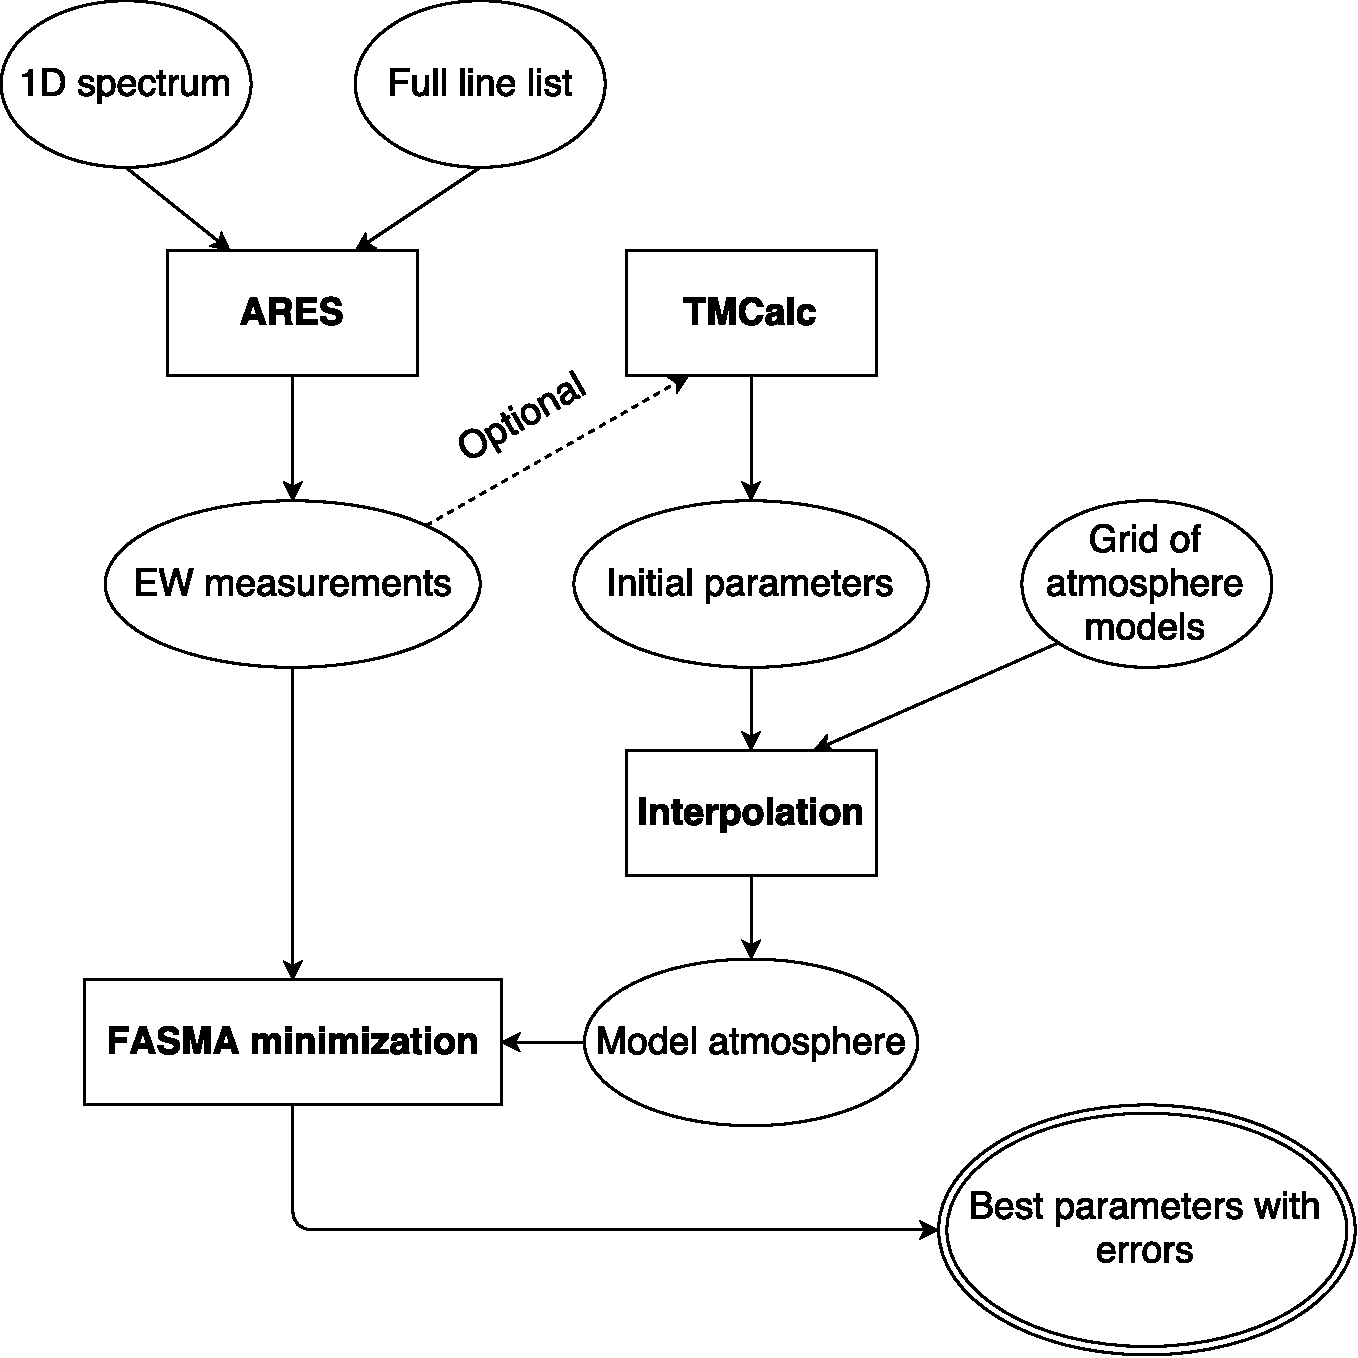
\includegraphics[width=1.0\linewidth,natwidth=700,natheight=650]{figures/FASMA_general.pdf}
    \caption{A general overview over FASMA from spectrum to parameters.}
    \label{fig:FASMA_general}
\end{figure}

There exist many minimization routines available in Python. The ones from the
SciPy ecosystem\footnote{\url{http://scipy.org}} are the most commonly known.
There are some advantages and disadvantages using proprietary minimization
routines. Advantages are that it is already written, and usually there is good
documentation for libraries such as SciPy. Disadvantages in this situation is,
that most minimization routines do not work well with vector functions returning
another vector:
\begin{align}
    f(\{T_\mathrm{eff}, \log g, [Fe/H], \xi_\mathrm{micro}\}) = \{a_\mathrm{EP}, a_\mathrm{RW}, \Delta\ion{Fe}, \ion{Fe}{I}\}. \label{eq:vector}
\end{align}
A work around this is to combine the criteria into one single criterion by e.g.
adding them quadratically and minimize that expression instead. Thus we have a
vector function returning a scalar:
\begin{align}
    f(\{T_\mathrm{eff}, \log g, [Fe/H], \xi_\mathrm{micro}\}) &= \sqrt{a_\mathrm{EP}^2 + a_\mathrm{RW}^2 + \Delta\ion{Fe}{}^2}. \label{eq:scalar}
\end{align}
The minimization routines are also not physical in the sense that they are not
written for the problem. These two disadvantages were an incitement for writing
a minimization routine specific for the problem at hand. This also allow us to
minimize the more complicated expression in Equation~\ref{eq:vector}. Here is
how it works:

\begin{enumerate}
    \item Run MOOG once with user defined initial parameters (default is
          solar) and calculate $a_\mathrm{EP}$, $a_\mathrm{RW}$, and
          $\Delta$\ion{Fe}.
    \item Change the atmospheric parameters ($T_\mathrm{eff}$, $\log g$,
          [\ion{Fe}/\ion{H}], $\xi_\mathrm{micro}$) according to the size of the
          indicator. A parameter is only changed if it is not fixed.
    \begin{itemize}
        \item $a_\mathrm{EP}$: Indicator for $T_\mathrm{eff}$. If this value
              is positive, then increase $T_\mathrm{eff}$. Decrease
              $T_\mathrm{eff}$ if $a_\mathrm{EP}$ is negative.
        \item $a_\mathrm{RW}$: Same as above but for $\xi_\mathrm{micro}$.
        \item $\Delta$\ion{Fe}{}: Positive $\Delta$\ion{Fe}{} means $\log g$
              should be decreased and vice versa.
        \item $[\ion{Fe}{}/\ion{H}{}]$ is changed to the output
              $[\ion{Fe}{}/\ion{H}{}]$ in each iteration.
    \end{itemize}
    \item If the new set of parameters have already been used in a previous
          iteration, then change them slightly. This is done by drawing a random
          number from a Gaussian distribution with a mean at the current value
          and a sigma equal to the absolute value of the indicator. For $T_\mathrm{eff}$
          the new value would be a random draw from
          $f(x|T_\mathrm{eff,old},a_\mathrm{EP}^2) = \frac{1}{\sqrt{2\pi a_\mathrm{EP}^2 }}e^{-\frac{(x - T_\mathrm{eff,old})^2 } {2 a_\mathrm{EP}^2} }$
          and similar for the other atmospheric parameters using the appropriate
          indicators.
    \item Calculate a new atmospheric model by interpolating a grid of models
          so we have the requested parameters and run MOOG once again.
    \item For each iteration save the parameters used and the quadratic sum of
          the indicators.
    \item Check for convergence, i.e. if the indicators are below or equal
          to the empirical constraints chosen. If we do not reach convergence,
          then return the best found parameters. The best found parameters,
          when convergence are not reached, are chosen when the quadratic sum
          of the indicators are smallest.
\end{enumerate}
This whole process is schematically shown in Figure~\ref{fig:FASMA_general} and
the minimization routine itself in Figure~\ref{fig:FASMA_minimization}. by
minimizing Equation~\ref{eq:vector} rather than Equation~\ref{eq:scalar} we can
much faster reach convergence, since we know in which direction we must change
the atmospheric parameters. The stepping in parameters follows these simple
empirical equations, where we add the right side (sign change according to the
sign of the indicator) to the left side:
\begin{align}
    T_\mathrm{eff}     &: \SI{2000}{K} \cdot a_\mathrm{EP}   \\
    \xi_\mathrm{micro} &: \SI{1.5}{km/s} \cdot a_\mathrm{RW} \\
    \log g             &: -\Delta\ion{Fe}.
\end{align}
The metallicity is corrected at each step so the input metallicity matches that
of the output metallicity of the previous iteration. The functional form
(linear) for changing the parameters were found by changing one parameter, e.g.
$T_\mathrm{eff}$, while keeping the other parameters fixed at their convergence
values using the Sun as an example. A linear fit was applied to $T_\mathrm{eff} -
T_\mathrm{eff,0}$ vs. $a_\mathrm{EP}$ in order to get the slope (\SI{2000}{K}
for $T_\mathrm{eff}$). Since we ignore all interdependencies between the
parameters, we lower the slopes found a little and arrived to the very simple
equations above. By empirically determining how the atmospheric parameters
should be changed in each iteration, we are able to swiftly reach closer to the
convergence value.

The error estimates are based on the same method presented in
\citet{Gonzalez2000}, which is also described in detail in
\citet{Santos2003,Andreasen2016}.

\begin{figure}[tpb]
    \centering
    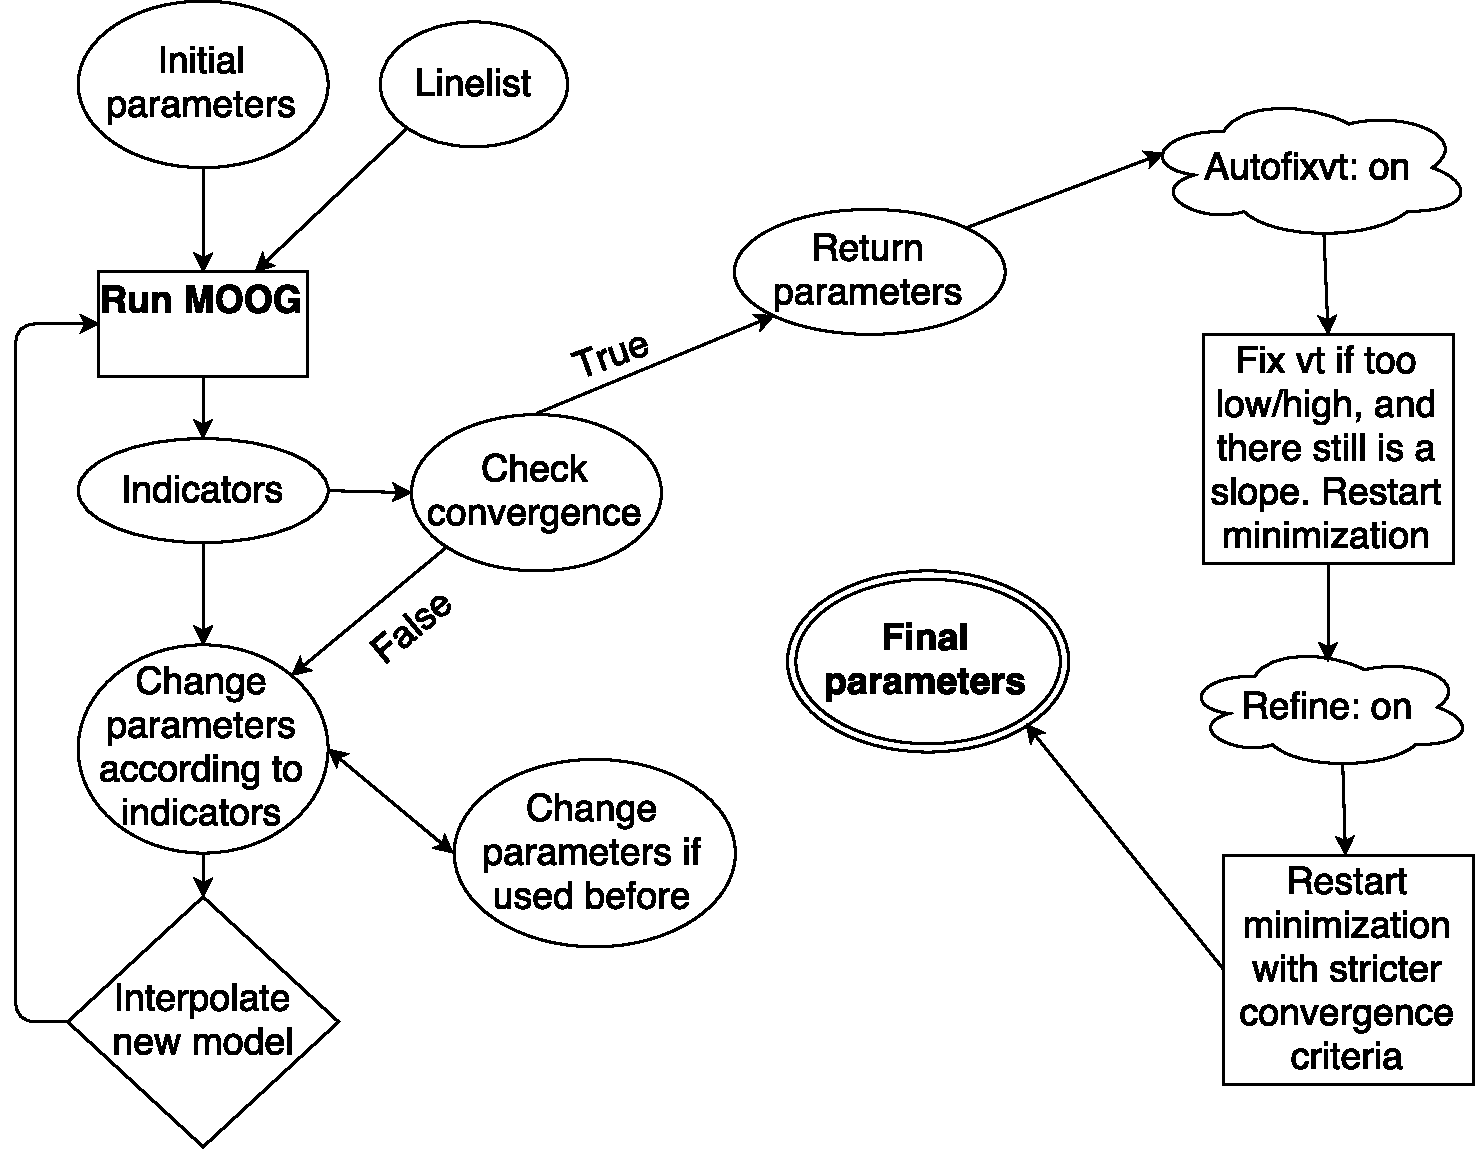
\includegraphics[width=1.0\linewidth,natwidth=700,natheight=650]{figures/FASMA_minimization.pdf}
    \caption{A schematic overview over the minimization for FASMA with the
    EW method.}
    \label{fig:FASMA_minimization}
\end{figure}

By using the indicators like this, we can reach convergence in a fast way.
Typical calculation time for an FGK dwarf with a high quality spectrum is around
$\SI{2}{min}$.

\subsubsection{Options}
\label{subs:EWoptions}
It is possible to run the EW method with a set of different options which
are described here.

\begin{itemize}
    \item \emph{fixteff}: Fix $T_\mathrm{eff}$ and derive the other parameters.
          Same is available for $\log g$ (\emph{fixlogg}), [\ion{Fe}/\ion{H}]
          (\emph{fixfeh}), and $\xi_\mathrm{micro}$ (\emph{fixvt}). One or more
          parameters can be fixed. When one or more parameters are fixed, the
          corresponding indicator will be ignored for each iteration, thus the
          parameter itself will not be changed.
    \item \emph{outlier}: Remove a spectral line(s) after the the minimization
          is done, if the abundance of this spectral line is more than $3\sigma$
          away from the average abundance of all the lines. After the removal
          of outlier(s) the minimization routine restarts. The options are to
          remove all outliers above $3\sigma$ once or iteratively, or remove one
          outlier above $3\sigma$ once or iteratively.
    \item \emph{autofixvt}: If the minimization routine does not converge and
          $\xi_\mathrm{micro}$ is close to 0 or 10 with a significant
          $a_\mathrm{RW}$ (numerically bigger than 0.05), then fix
          $\xi_\mathrm{micro}$. This option was added since we saw this
          behaviour in some cases. The solution was typically to restart the
          minimization manually with $\xi_\mathrm{micro}$ fixed. If
          $\xi_\mathrm{micro}$ is fixed it is changed at each iteration
          according to an empirical relation. For dwarfs it follows the one
          presented in \citet{Tsantaki2013} and for giants it follows the one
          presented in \citet{Adibekyan2015}.
    \item \emph{refine}: After the minimization is done, run it again from the best
          found parameters but with more strict criteria. If this option is set,
          it will always be the last step (after removal of outliers). The
          convergence criteria can be changed by the user, but we recommend
          using the defaults provided above.
    \item \emph{tmcalc}: Use TMCalc \citep{Sousa2012} to fast estimate the
          $T_\mathrm{eff}$ and $[\ion{Fe}/\ion{H}]$ using the raw output from
          ARES. We then assume solar surface gravity ($\SI{4.44}{dex}$) and
          estimate $\xi_\mathrm{micro}$ based on an empirical relation (see above).
\end{itemize}

For the optical we use the line list presented in \citet{Sousa2008a}. However,
this line list does not work well for cool stars. This was fixed in
\citet{Tsantaki2013} by removing some lines from \citet{Sousa2008a}. For stars
cooler than \SI{5200}{K} we automatically rederive the atmospheric parameters
after removing lines so the line list resemble that of \citet{Tsantaki2013}. The
line list for the NIR is also available \citep{Andreasen2016}.

All restarts of the minimization routine are done at the last found best
parameters as initial conditions.


\subsection{Abundance method}
\label{sub:Abundance_method}

FASMA calculates element abundances for 12 different elements (\ion{Na}{},
\ion{Mg}{}, \ion{Al}{}, \ion{Si}{}, \ion{Ca}{}, \ion{Ti}{}, \ion{Cr}{},
\ion{Ni}{}, \ion{Co}{}, \ion{Sc}{}, \ion{Mn}{}, and \ion{V}{}) from spectral
lines determined in \citet{Neves2009} and \citet{Adibekyan2012}. It also
includes three ionized elements: \ion{Cr}{II}, \ion{Sc}{2}, and \ion{Ti}{II}.
The abundances are derived using MOOG in the same way as described above for
\ion{Fe}{}. The atomic data were calibrated with the Sun as reference and solar
abundances from \citet{Anders1989}. The EWs are measured automatically with the
ARES driver of FASMA. The element abundance of each line is derived using the
atmospheric parameters of the stars obtained from the previous step. The final
element abundance is calculated from the weighted mean of the abundances
produced by all lines detected for a given element as described in
\citet{Adibekyan2015b}.


\subsection{Testing FASMA}
\label{sub:Testing_FASMA}

To test the derivation of stellar parameters implemented in FASMA we derive
parameters from the 582 sample by \citet{Sousa2011}. We use ARES to measure the
EWs. ARES can give an estimate on the SNR by analyzing the continuum in certain
intervals. For solar type stars the following intervals are working well:
\SIrange{5764}{5766}{\angstrom}, \SIrange{6047}{6053}{\angstrom}, and
\SIrange{6068}{6076}{\angstrom}. From the estimated SNR, ARES can give an
estimate on the very important \emph{rejt} parameters
\citep[see][for more information]{Sousa2015a}. After measuring the EWs with ARES,
we use the FASMA minimization routine described in Section~\ref{sub:EW_method}
to determine the stellar atmospheric parameters. The results are presented in
Figure~\ref{fig:FASMATest} which shows $T_\mathrm{eff}$, $\log g$,
[\ion{Fe}/\ion{H}], and $\xi_\mathrm{micro}$ for FASMA against those of
\citet{Sousa2011}.

\begin{figure*}[tpb]
    \centering
    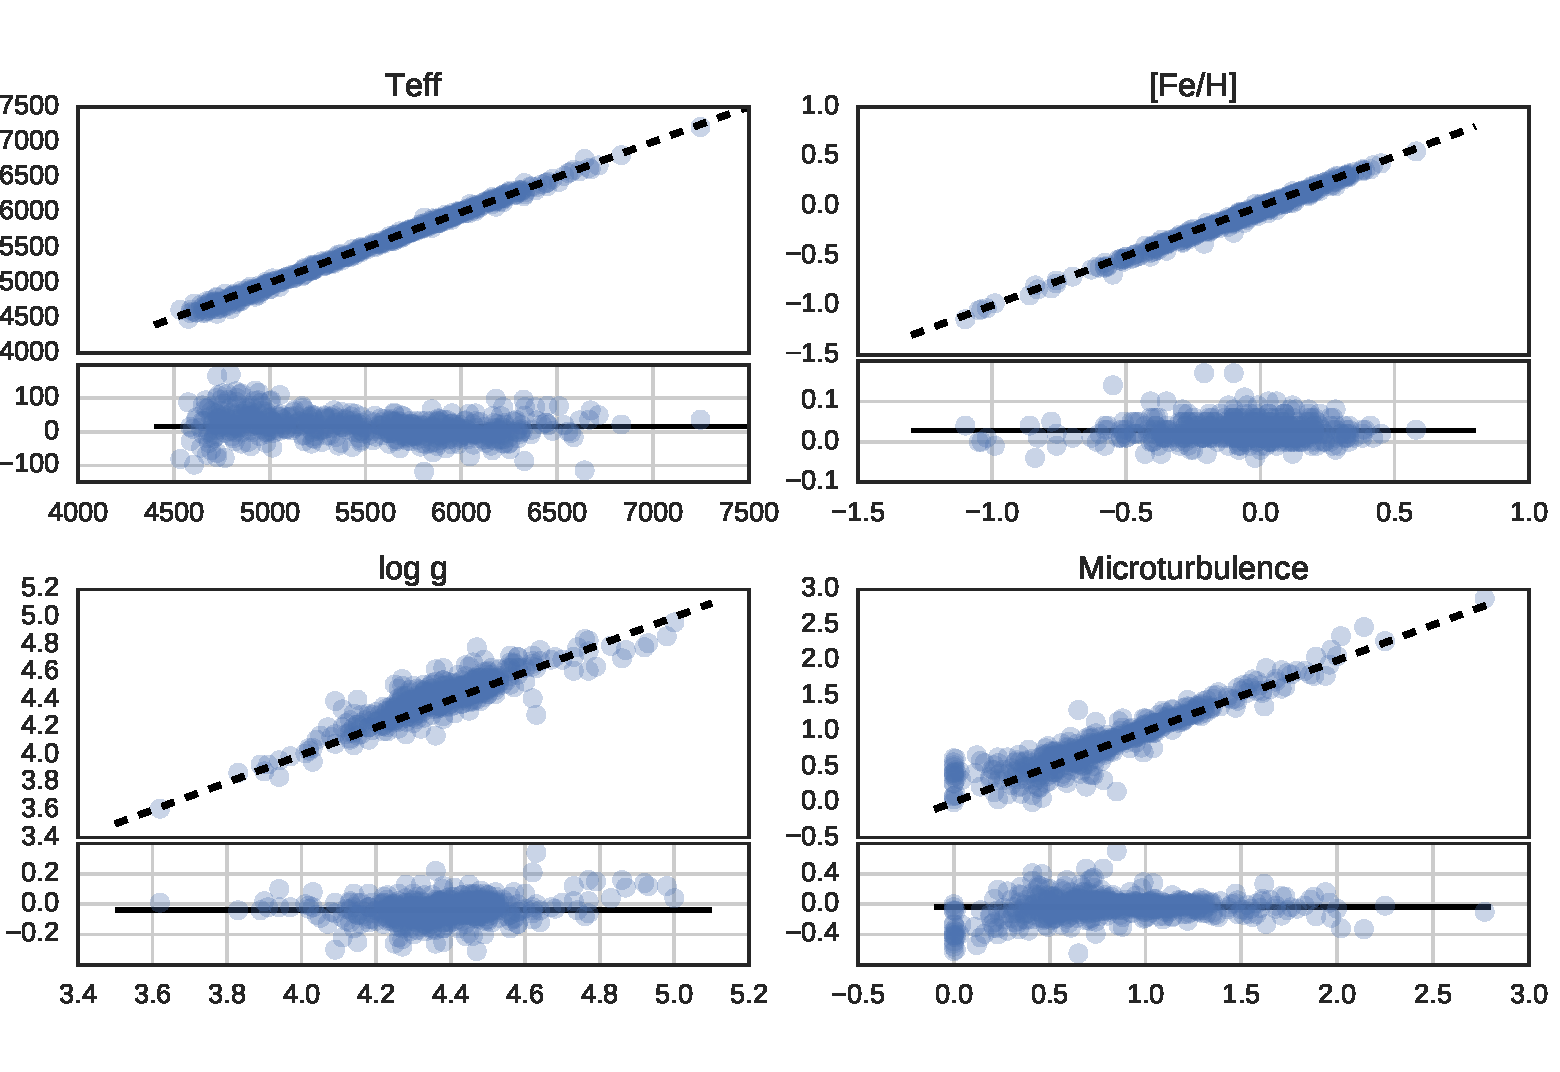
\includegraphics[width=1.0\linewidth,natwidth=750,natheight=500]{figures/FASMATest.pdf}
    \caption{Stellar atmospheric parameters derived by FASMA compared
    to the sample by \citet{Sousa2011}. The x-axis in all plots show the results
    from FASMA while the y-axis is the parameters derived by \citet{Sousa2011}.}
    \label{fig:FASMATest}
\end{figure*}

The sample contains stars with $T_\mathrm{eff}$ too cold for the line list used.
As described in Section~\ref{sub:EW_method} we should then convert the line list
by \citet{Sousa2008a} to the line list presented in \citet{Tsantaki2013}.
However, since this line list was not available when \citet{Sousa2011} derived
parameters, we do not make this change in order to make a fair comparison for
FASMA.

The mean of the difference between parameters from \citet{Sousa2011} and those
by FASMA are presented in Table~\ref{tab:FASMATest}.

\begin{table}[htb!]
    \caption{The difference in derived parameters by \citet{Sousa2011}
    and FASMA. Second column is the mean difference with EWs measured by
    ARES in FASMA, while the third column is the mean difference using
    20 randomly stars with the exact same EWs from \citet{Sousa2011}.}
    \label{tab:FASMATest}
    \centering
    \begin{tabular}{lrr}
      \hline\hline
      Parameter             &  Mean difference         & Same line list        \\
      \hline
      $T_\mathrm{eff}$      &  $\SI{16(36)}{K}$        & $\SI{21(11)}{K}$      \\
      $\log g$              &  $\num{-0.04(7)}$        & $\num{-0.007(9)}$     \\
      $[\ion{Fe}/\ion{H}]$  &  $\num{0.03(2)}$         & $\num{0.004(9)}$      \\
      $\xi_\mathrm{micro}$  &  $\SI{-0.04(14)}{km/s}$  & $\SI{0.04(2)}{km/s}$  \\
      \hline
    \end{tabular}
\end{table}

The comparison is very consistent as expected and the small offsets are within
the errors except for metallicity. This can be due to different versions of
MOOG, measured line lists (i.e. using slightly different settings/version of
ARES to measure the EWs), interpolation of atmosphere grid, and minimization
routine. Most likely the difference will be due to different used \emph{rejt}
parameters in ARES, which can alter the EWs systematically and hence the
metallicity. We therefore randomly selected 20 stars with different
$T_\mathrm{eff}$ and used the EWs directly from \citet{Sousa2011} to derive
parameters. The results are presented in the last column of
Table~\ref{tab:FASMATest}. We note that the $\log gf$ values from the original
line lists by \citet{Sousa2011}, which used the MOOG 2002 version, were not
changed for the 2014 version of MOOG. This might lead to some errors as well.
However, the offsets are very small and compatible with the errors on parameters
normally obtained from high quality spectra.


\subsection{Web interface}
\label{sub:Web interface}

We provide a web interface for FASMA. In the web interface it is possible to use
some of the line list provided with FASMA to measure EWs of a spectrum. The
spectrum is expected to be in a 1D format with the wavelength information stored
in the header keys, CRVAL1 for the minimum wavelength, CDELT1 for the stepping
in wavelengths, and NAXIS1 for the number of points. This can be used for all
the available FASMA methods described above. ARES does the normalization, but
best results are found when the spectrum is properly reduced (removal of cosmic
rays, normalized, etc.).

The web interface can be found at the following link
\url{http://www.iastro.pt/fasma}, where more information are available on each
of the driver. The user must provide an email. This is only used to send the
results after the calculations.


\section{SWEET-Cat update}

\subsection{Data}
\label{sec:data}
In this paper we derived parameters for a sample of 50 stars, 43 were observed
by our team using the UVES/VLT \citep{UVES}, FEROS/2.2m telescope in La Silla
\citep{FEROS}, and FIES/NOT \citep{FIES} spectrographs. The rest (23) spectra
were found in various archives. We use spectra from HARPS/3.6m telescope in La
Silla \citep{HARPS} and ESPaDOnS/CFHT \citep{ESPADONS}. Some characteristics of
the spectrographs are presented in Table~\ref{tab:instruments} with the mean SNR
for the spectra used. The SNR for each star can be seen in
Table~\ref{tab:results} along with the atmospheric parameters of the stars. The
SNR is measured automatically by ARES, but we note that ARES smooth the spectra
before measuring the SNR, hence it is listed higher than the actual SNR. These
50 stars are confirmed exoplanet hosts listed in SWEET-Cat. However, these
belonged to the list of stars that have not been analysed by our team. We
therefore increase the amount of stars analyzed in a homogeneous way, which is
the goal of SWEET-Cat.

We obtain the spectra with the highest possible resolution for a given
spectrograph, and in cases with multiple observations, we include all unless a
spectrum is close to the saturation limit for a given spectrograph. For multiple
spectra, we combine them after first correcting the radial velocity (RV) and
using a sigma clipper to remove cosmic rays. The individual spectra are then
combined to a single spectrum for a given star to increase the SNR. This single
spectrum is used in the analysis described below. For most of the spectra in the
archive included here, several spectra were combined as described above, while
for the observations dedicated to this work, the spectrum would be a single
spectrum, or in cases of faint stars, it would be observed a few times to reach
the desired SNR. This is mostly due to the difference in science cases behind
the observations. E.g. the HARPS spectra were used for RV monitoring or follow
up of the exoplanet(s), while the UVES spectra were used for characterisation of
stellar parameters.

\begin{table}[htb!]
    \caption{Spectrographs used for this paper with their spectral resolution,
             wavelength coverage, and mean SNR from the spectra used.}
    \label{tab:instruments}
    \centering
    \begin{tabular}{llll}
      \hline\hline
      Spectrograph & Resolution & Spectral range              &   Mean SNR  \\
      \hline
      HARPS        &    115 000 & $\SIrange{378}{691}{nm}$    &   642       \\
      UVES         &    110 000 & $\SIrange{480}{1100}{nm}$   &   212       \\
      ESPaDOnS     &     81 000 & $\SIrange{370}{1050}{nm}$   &   775       \\
      FIES         &     67 000 & $\SIrange{370}{730}{nm}$    &   763       \\
      FEROS        &     48 000 & $\SIrange{350}{920}{nm}$    &   208       \\
      \hline
    \end{tabular}
\end{table}



\subsection{Analysis}
\label{sec:results}
Here we present the sample of 50 stars. We were unable to derive parameters for
{16 (not included in the 50)} of our targets. For example, HD77065 is a
spectroscopic binary according to \cite{Pourbaix2004}, and the spectrum is
contaminated with the companion star. This make EW measurement very difficult,
hence we exclude it from the sample of collected spectra.

Moreover we were not able to successfully derive parameters with this method for
Aldebaran, a well known red giant star. Even though spectra of good quality are
available for a bright star like Aldebaran, this spectral type is intrinsically
difficult to analyse due to the molecular absorption that arise in the optical
region at low $T_\mathrm{eff}$ (\SI{4055}{K} is listed in SWEET-Cat as measured
by \citet{Hatzes2015}). The fact that we are not able to derive parameters for
Aldebaran is not a big concern, since it is well studied with other techniques,
and we can trust the parameters already listed in SWEET-Cat.

In total, we removed 16 stars from our sample since the parameters for
these stars did not converge during the minimization procedure. The
$T_\mathrm{eff}$ for these stars is either too hot, above \SI{7500}{K} or
too cold, below \SI{4000}{K} for the EW method to work.

The remaining 50 stars are presented in Table~\ref{tab:results}. Note that we
apply a correction to the spectroscopic $\log g$ based on asteroseismology as
found by \citet{Mortier2014}. We only use this correction for FGK dwarf stars,
i.e. between $\SI{4800}{K}\leq T_\mathrm{eff} \leq \SI{6500}{K}$ and $\log
g\geq4.2$. For stars with a $\log g$ lower than this limit we do not apply the
corrections, and if the $\log g$ change to below this limit after the
correction, we go back to use the spectroscopic $\log g$ again. The correction
for $\log g$ depends on both $T_\mathrm{eff}$ and $\log g$. The correction can
be up to 0.5 dex, depending on the $T_\mathrm{eff}$.

We present a Hertzprung-Russel diagram (HRD) of our sample in
Figure~\ref{fig:HRD}, which is made with a tool for post processing the results
saved to a table by FASMA.

\begin{figure}[tpb]
    \centering
    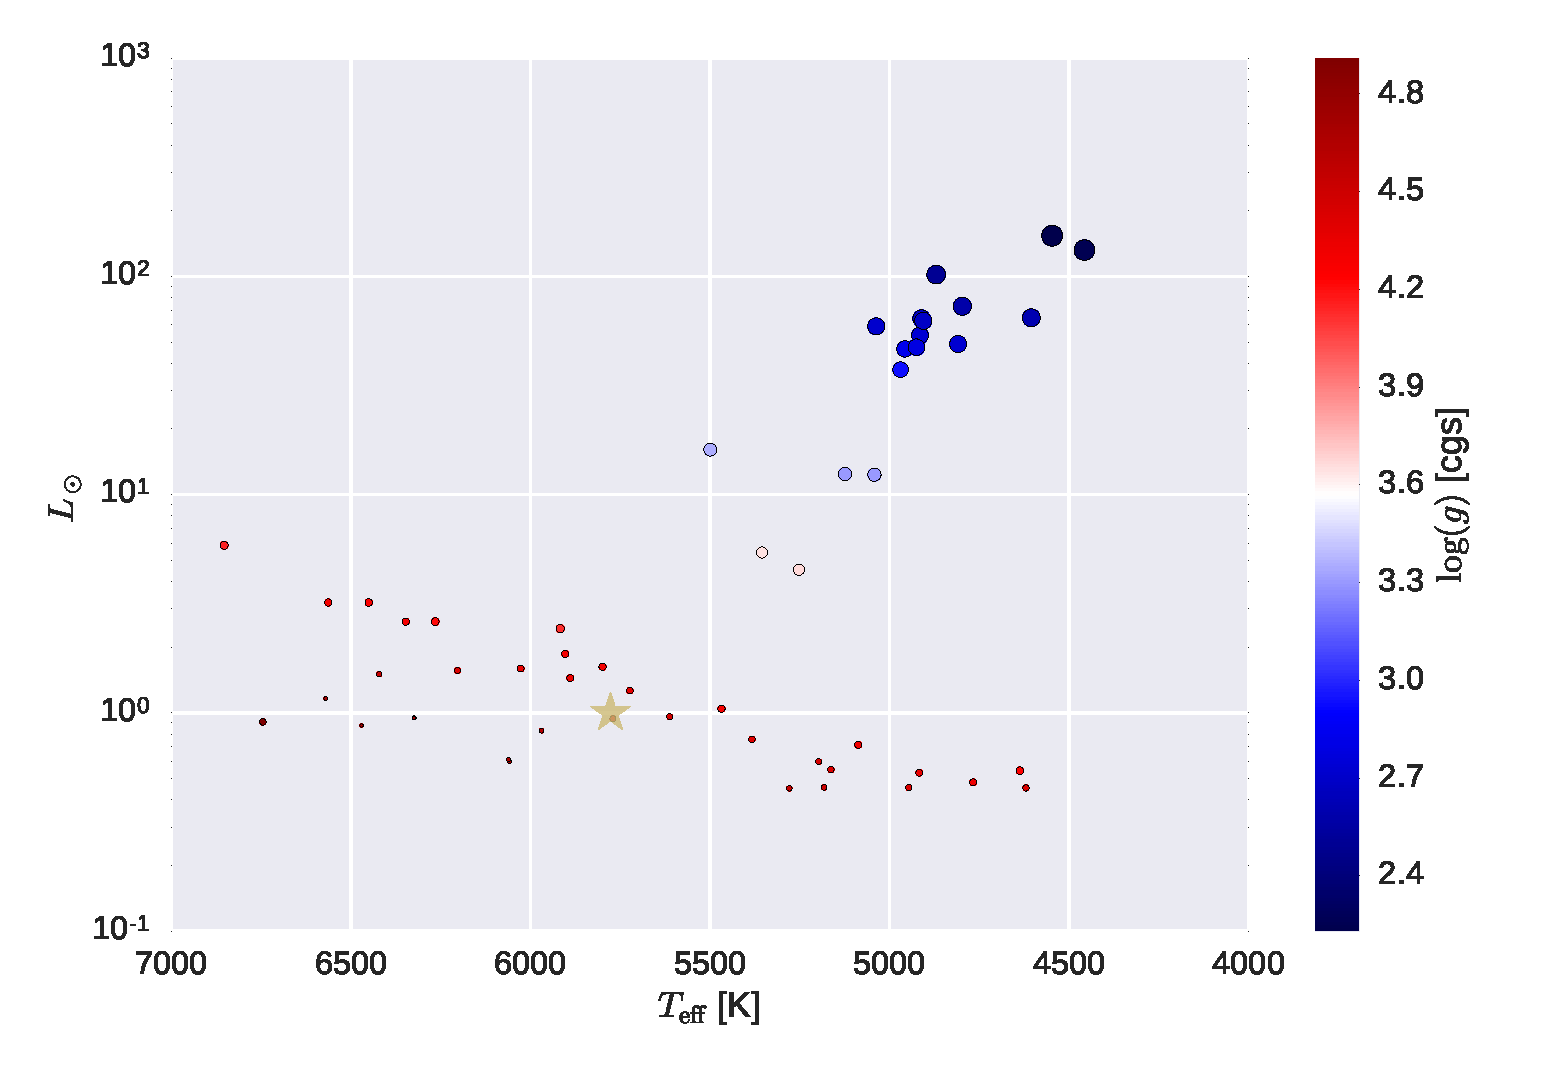
\includegraphics[width=1.0\linewidth,natwidth=440,natheight=290]{figures/HR.pdf}
    \caption{Hertzprung-Russel diagram of our sample with the Sun as a green
    star. The size of the points represents the $\log g$, with bigger points
    being smaller $\log g$ (giants), and vice versa. The colour code show the
    same as the size. Red points are the dwarfs, while yellow points are the
    giants.}
    \label{fig:HRD}
\end{figure}

The new atmospheric parameters are presented in Figure~\ref{fig:update} against
the literature values we listed previously in SWEET-Cat. The red points showing
the location of the outliers as discussed below, are mainly visible outliers for
$\log g$ at the low end, i.e. for the sub-giant to giant stars. The old
parameters are listed in Table~\ref{tab:oldSC}. Among 2437 stars discovered to
be a planet hosts, 21\% of these stars have been analyzed in the homogeneous way
as described in this work. We note that the limiting factor at the moment for
increasing the sample of stars analyzed in the homogeneous way is the magnitude
of the planet hosts. There have been found many planet hosts with space missions
as \emph{Kepler} and \emph{CoRoT} using the transiting method. Most of these
stars are faint and thus making them observationally expensive for the
spectroscopic analysis required here. For stars brighter than magnitude 12 the
completeness, i.e. the stars analyzed in a homogeneous way compared to the ones
we did not analyze yet, is up to 77\% now while it is at 85\% for exoplanet
hosts brighter than magnitude 10.

\begin{figure*}[tpb]
    \centering
    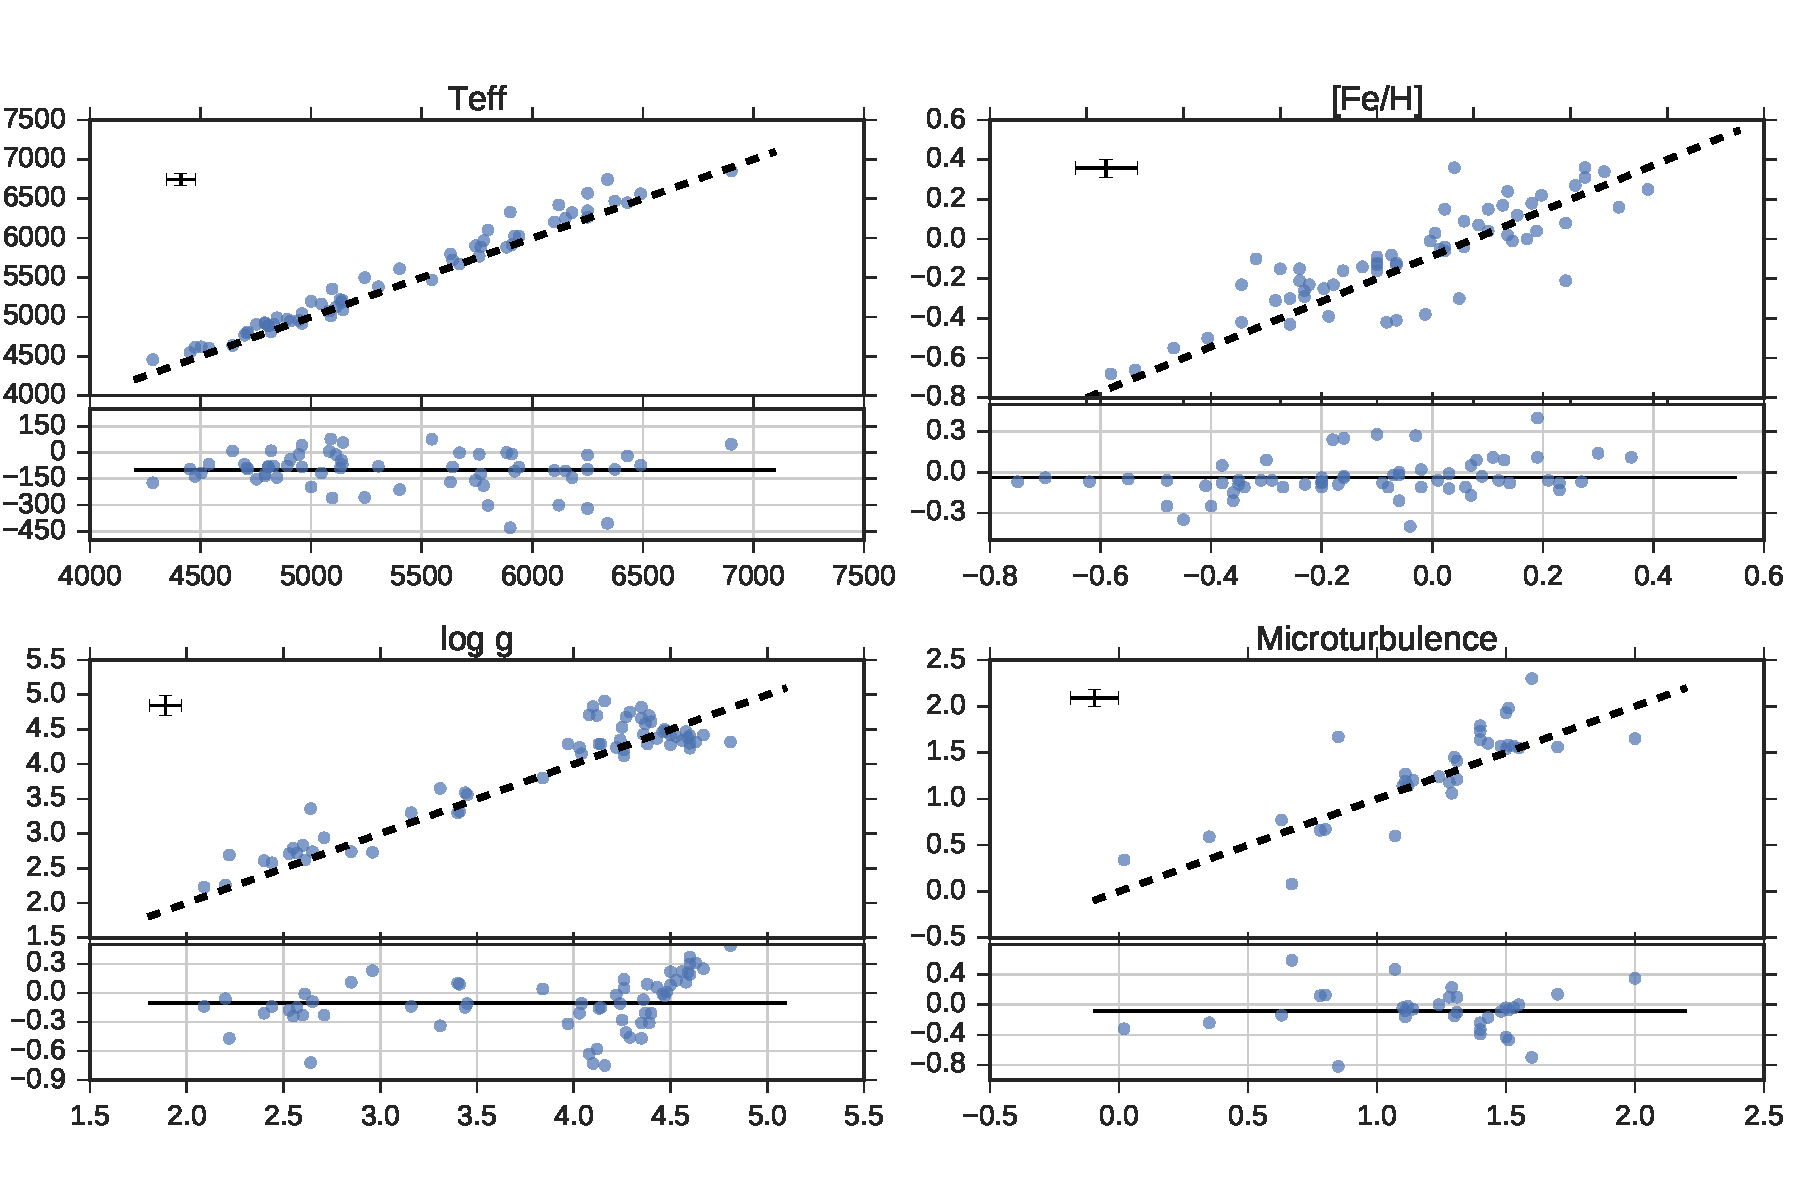
\includegraphics[width=1.0\linewidth,natwidth=870,natheight=580]{figures/update.pdf}
    \caption{Atmospheric parameters of the updated planet host stars. The x-axis
    are the previous values in SWEET-Cat (see Table~\ref{tab:oldSC}), while the
    y-axis is the new updated values. In the upper left corner of each of the
    four plots we show the typical error on the parameters. The red points
    are outliers as discussed in Section~\ref{sec:Discussion}.}
    \label{fig:update}
\end{figure*}

The metallicity distribution for all the planet host stars are important to
understand e.g. planet formation. We present a distribution in
Figure~\ref{fig:distribution}. The sample is divided in two, for all planet
hosts in SWEET-Cat, and for stars brighter than 12 V magnitude. Stars dimmer are
mainly observed with the \emph{Kepler} space mission. These dim stars are very
time consuming, and hence expensive to observe. Out of the 2437 stars in
SWEET-Cat, 664 of them are brighter than 12 V magnitude. We note that more than
1500 of the stars does not have a V magnitude. The majority are stars observed
with \emph{Kepler}. Our group have analyzed 563 stars in SWEET-Cat including the
50 stars presented in this work.


\begin{figure}[tpb]
    \centering
    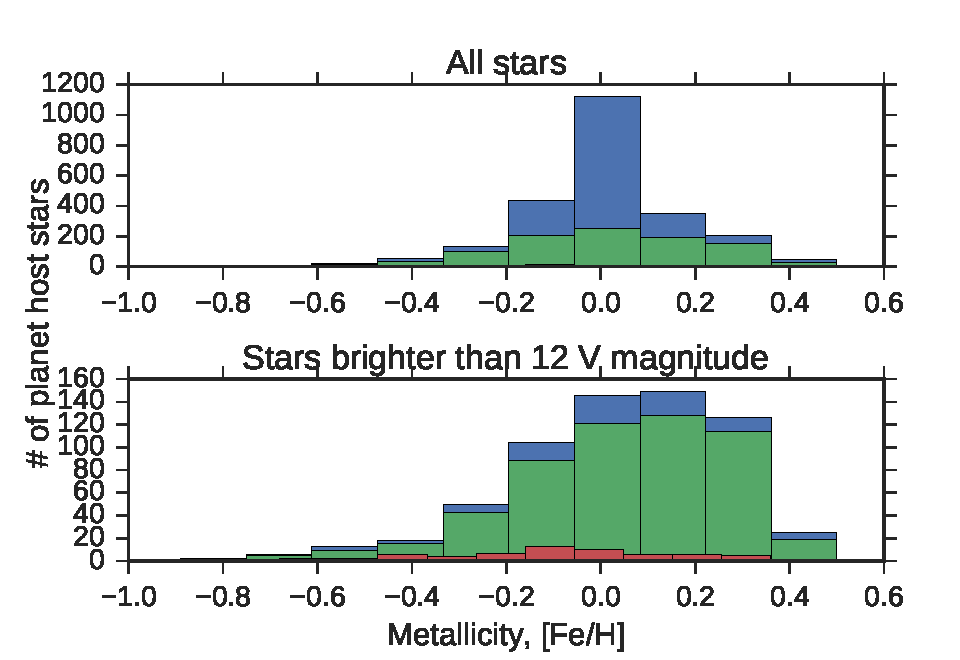
\includegraphics[width=1.0\linewidth,natwidth=450,natheight=300]{figures/metallicityDistribution.pdf}
    \caption{The metallicity distribution. In the \emph{upper} plot we see all
             stars (logarithmic scale) in SWEET-Cat, divided in three. Blue
             (the largest distribution) are all stars available in SWEET-Cat,
             green (the middle distribution) are the stars with homogenity flag
             1, i.e. analyzed using the method described in this paper, red
             (the smallest distribution) are all new stars added from this
             paper. The \emph{lower} plot show a 12 V magnitude cut to exclude
             stars which are currently unavailable spectroscopically.}
    \label{fig:distribution}
\end{figure}



\subsection{Discussion}
\label{sec:Discussion}
We compute radius and mass of all the 50 new stars updated in SWEET-Cat (even
the ones whose parameters may not be reliable, in order to be complete) using
the empirical formula presented in \citet{Torres2010}. Some of the stars have
radius derived from different methods, usually from isochrones. These radii
generally show a good correlation with radii derived from \citet{Torres2010} if
the literature parameters of $T_\mathrm{eff}$, $\log g$, and
$[\ion{Fe}/\ion{H}]$ are used. However, if we compare with the new radius
derived using the parameters presented here, the results can differ up to 65\%.
We show in Figure~\ref{fig:RR} how the radius calculated from \citet{Torres2010}
differ between the literature atmospheric parameters and the new homogeneous
atmospheric parameters presented here. We note that stellar radii is provided by
many of the authors from different discovery papers, but we chose to compare the
atmospheric parameters via the derivation of the stellar radius as described
above, rather than compare the stellar radii from different methods.

\begin{figure}[tpb]
    \centering
    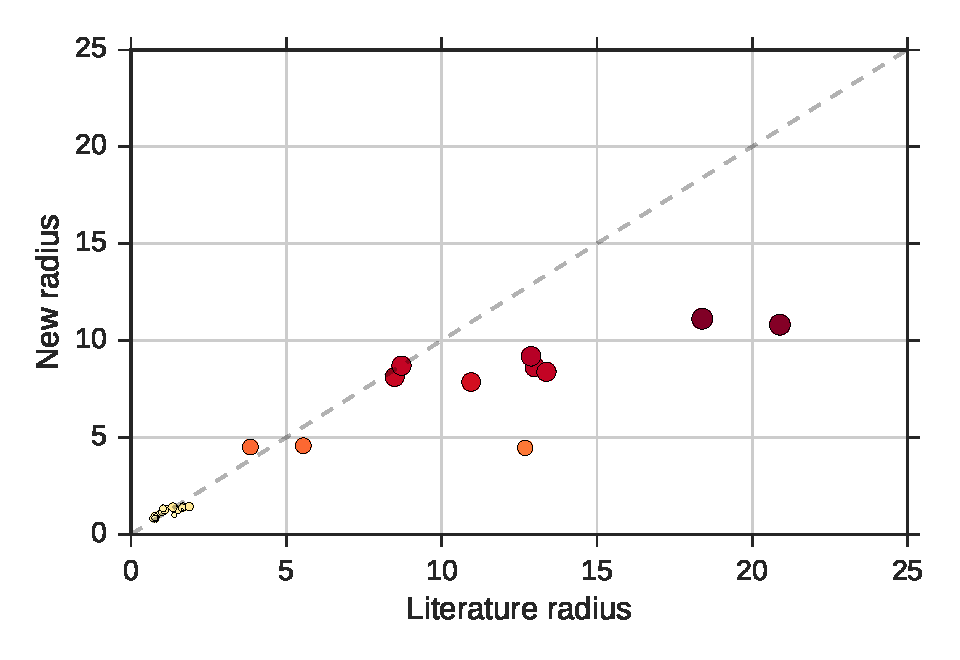
\includegraphics[width=1.0\linewidth]{figures/radiusVSradius.pdf}
    \caption{The stellar radius on both axis calculated based on \citet{Torres2010}.
    For the x-axis we show the stellar radius based on the atmospheric parameters
    from the literature, while the y-axis is from the new homogeneous parameters
    presented here. The colour and size present the surface gravity. This clearly
    shows that the disagreement is biggest for more evolved stars.}
    \label{fig:RR}
\end{figure}

In the subsections below we discuss the systems (seven stars, eight exoplanets)
where the radius or mass of the stars changes more then 25\% and how this
influences the planetary parameters. The changes in radius for a star is
primarily due to changes in $\log g$, which can be used as an indicator of the
evolutionary stage of a star.

We rederive the planetary radius, mass and semi-major axis when possible
following the three simple scaling relations based on Newton's law of gravity
\citep{Newton1687} for deriving mass and distance and simple geometry for radius
\citep[see e.g.][]{Torres2008}.:

\begin{align}
    M_\mathrm{pl,new} &= \left(\frac{M_\mathrm{\ast,lit}}{M_\mathrm{\ast,new}}\right)^{-2/3} M_\mathrm{pl,lit}  \\
    R_\mathrm{pl,new} &= \left(\frac{R_\mathrm{\ast,lit}}{R_\mathrm{\ast,new}}\right) R_\mathrm{pl,lit} \\
    a_\mathrm{pl,new} &= \left(\frac{M_\mathrm{\ast,lit}}{M_\mathrm{\ast,new}}\right)^{1/3} a_\mathrm{pl,lit},
\end{align}
where subscript "lit" denotes the value from the literature which we compare
with, subscript "new" is finally the new computed values, subscript "pl" is
short for planet, and last subscript "$\ast$" is short for star. $M$, $R$, and
$a$ are mass, radius, and semi-major axis, respectively. Note that for the
literature values, we use the values reported directly from the literature, and
not the derived radius and mass from \citet{Torres2010}. To identify outliers,
we compare radii and masses derived from \citet{Torres2010} since this is a
measure of how the atmospheric parameters have changed.

\subsubsection{HAT-P-46}
\label{sub:HAT-P-46}
HAT-P-46 has two discovered exoplanets according to \citet{Hartmann2014}. The
outer planet HAT-P-46 c is not transiting hence we do not have any radius for
this planet. The results we present in this paper for this star comes from
UVES/VLT data with a SNR at 208. \citet{Hartmann2014} derives the following
spectroscopic parameters: $T_\mathrm{eff}=\SI{6120(100)}{K}$, $\log
g=4.25\pm0.11$, and $[\ion{Fe}/\ion{H}]=0.30\pm0.10$. We note that for this star
the asteroseismic correction we apply as mentioned in Section~\ref{sec:results}
results in a corrected $\log g$ below 4.2dex, so we end up using the
spectroscopic $\log g$ for this star.

If we derive the mass and radius of HAT-P-46 b with our new parameters, we
obtain the following: $R_\mathrm{pl} = 0.93R_J$, while \citet{Hartmann2014}
derived $R_\mathrm{pl} = 1.28R_J$. We see no change in mass
(\citet{Hartmann2014} found $M_\mathrm{pl}=0.49M_J$), however there is a
decrease in the radius, and we end up with a more dense planet,
$\rho_\mathrm{pl}=\SI{0.76}{g/cm^3}$ from $\rho_\mathrm{pl}=\SI{0.28\pm0.10}{g/cm^3}$.

As the secondary companion does not transit we only have a limit on the minimum
mass for this planet. Here we get: $M\sin i_\mathrm{pl} = 1.97M_J$,
\citet{Hartmann2014} presented $M\sin i_\mathrm{pl} = 2.00M_J$, so a very
small change as expected.


\subsubsection{HD 120084}
\label{sub:HD_120084}
The exoplanet orbiting this star with a period of 2082 days and a quite
eccentric orbit at 0.66 was discovered by \citet{Sato2013}. Atmospheric
parameters were derived by \citet{Takeda2008} using a similar method as
described in this paper. The spectra they analyzed however, was not of as high
quality as used here. Using the HIDES spectrograph at the 188cm reflector at
NAOJ \citet{Takeda2008} reported an average SNR for their sample of 100-300 at a
resolving power of 67 000. We used data from ESPaDOnS with a resolving power of
81 000, and with a SNR for this star of 850. With our new parameter we obtain a
slightly lower stellar mass for the star at $1.93M_\odot$ compared to
$2.39M_\odot$ obtained by \cite{Takeda2008}, hence the minimum planetary mass is
also decreased slightly from $m_\mathrm{pl}\sin i=4.5M_J$ to $m_\mathrm{pl}\sin
i=3.9M_J$. We see a decrease in the stellar radius by 28\% from $9.12R_\odot$ to
$7.81R_\odot$. Since there are no observations of the planet transiting, the
planetary radius has not been computed.


\subsubsection{HD 233604}
\label{sub:HD_233604}
HD 233604 b was discovered by \citet{Nowak2013} while the atmospheric parameters
of the star were derived by \citet{Zielinski2012} with the same method as
described in this paper using the HRS spectrograph at HET with a resolving power
of 60 000 with a typical SNR at 200-250. We obtained the spectrum for this star
using the FIES spectrograph with a slightly higher resolution at 67 000, and
similar but also slightly higher SNR at 320 for this star.

This planet is in a very close orbit with a semi-major axis of $\sim 15R_\ast$
($R_\ast$ is the stellar radius) using the parameters from \citet{Nowak2013}.
With the updated parameters presented in this paper we see a slight increase in
the stellar mass from $1.5M_\odot$ to $1.9M_\odot$ and a decrease in stellar
radius from $10.5R_\odot$ to $8.6R_\odot$. This gives an increase of the semi
major axis to $\sim 21R_\ast$. Note that the correct stellar radii are used to
describe the semi-major axis in both cases.

The increase in stellar mass leads to an increase in the minimum planetary mass,
from $m_\mathrm{pl}\sin i=6.58M_J$ to $m_\mathrm{pl}\sin i=7.79M_J$.

\citet{Nowak2013} found a high \ion{Li}{} abundance at
$A(\ion{Li}{})_\mathrm{LTE}=1.400\pm0.042$ for this star speculating if this
star might have engulfed a planet. A more likely explanation is that this star
has not yet reached the first dredge-up process \citep{Nowak2013}. We found a
much lower value, $A(\ion{Li}{})_\mathrm{LTE}=0.92$ and hence we find the star
to not be \ion{Li}{} rich. The \ion{Li}{} abundance we find is in excellent
agreement with \citet{Adamow2014}. Even applying a NLTE correction as done in
\citet{Adamow2014} ($A(\ion{Li}{})_\mathrm{NLTE}=1.08$) this star is not
\ion{Li}{} rich.


\subsubsection{HD 5583}
\label{sub:HD_5583}
This exoplanet was discovered by \citet{Niedzielski2016} with an orbital period
of 139 days around a K giant. This exoplanet was discovered with the radial
velocity technique, and we do not have a planetary radius. The stellar
parameters were derived in a similar manner as presented here \citep[see][and
references therein]{Niedzielski2016} where our biggest disagreement is in the
surface gravity. We derive a 0.34 dex higher $\log g$ giving us a smaller
stellar radius (37\% smaller). The derived mass is 15\% higher which in turn
increases the minimum planetary mass from $m_\mathrm{pl}\sin i=5.78M_J$ to
$m_\mathrm{pl}\sin i=8.63M_J$. Even with the increase in mass, it is still
within the planetary regime for most inclinations as noted by
\citet{Niedzielski2016}.



\subsubsection{HD 81688}
\label{sub:HD81688}
This exoplanet was discovered by \citet{Sato2008} with the RV method. The host
star is a metal-poor K giant. The atmospheric parameters presented in
\citet{Sato2008} are obtained from the same method as presented in this paper,
and we have quite good agreement. Once again the big disagreement is in the
surface gravity where ours is 0.48 dex higher. Even though the stellar
parameters, and hence the planetary, do change, the radius and mass we derive
are not far from what is presented in the paper by \citet{Sato2008}. This is a
case where the star was marked as an outlier due to the comparison between the
radius and mass derived from \citet{Torres2010}.

The new stellar mass is the same as before, $2.1M_\odot$. The stellar radius
change from $13.0R_\odot$ to $10.8R_\odot$. Since a transit of this star has not
been observed and the stellar mass remains the same, we do not see any change in
the planetary parameters.

We note that this system is in an interesting configuration with a very close
orbit around an evolved star. This system, among others, have been subject
to work on planet engulfment \citep[see e.g.][]{Kunitomo2011}.


\subsubsection{HIP 107773}
\label{sub:HIP_107773}
The planetary companion was presented in \citet{Jones2015} as an exoplanet
around an intermediate mass evolved star. The stellar parameters were obtained
from the analysis by \citet{Jones2011} using the same method as presented here,
however with a different line list which might lead to some disagreements. For
this star we derive a higher $\log g$ at 2.83 dex compared to 2.60 dex, thus we
derive a slightly smaller star with $11.6R_\odot$ to $9.2R_\odot$ and
$2.4M_\odot$ to $2.1M_\odot$ for radius and mass of the star, respectively. The
other atmospheric parameters are very similar to those derived by
\citet{Jones2011}. This leads to a reduced minimum mass of the planetary
companion from $m\sin i=1.98M_J$ to $m\sin i=1.78M_J$. The planetary radius has
not been measured.



\subsubsection{WASP-97}
\label{sub:WASP-97}
The exoplanet orbiting WASP-97 was discovered by \citet{Hellier2014}. The host
star parameters were derived in a similar method as described in this paper
after co-adding several spectra from the CORALIE spectrograph. They reach a
SNR of 100 with a spectral resolution of 50 000. The parameters presented here
comes from the UVES spectrograph with a SNR of more than 200.

The parameters do not change much for this planet. The planetary mass is changed
from $m_\mathrm{pl}\sin i=1.32M_J$ to $m_\mathrm{pl}\sin i=1.37M_J$ and the
radius from $1.13R_J$ to $1.42R_J$. This does affect the density quite a lot,
changing from $\SI{1.13}{g/cm^3}$ to $\SI{0.59}{g/cm^3}$. This exoplanet is then
in the same category as Saturn with a density lower than water, however with a
size slightly larger than Jupiter.


\subsubsection{$\omega$ Serpentis (ome Ser)}
\label{sub:ome_Ser}
The exoplanet orbiting this star with a period of 277 days and an eccentric
orbit at 0.11 was also presented by \citet{Sato2013}. The atmospheric parameters
were derived in the same way as for HD 120084. We used data from FIES with a
resolving power of 67 000, and with a SNR for this star of 1168. With our new
parameters we obtain a slightly higher stellar mass for the star at
$2.19M_\odot$ compared to $2.17M_\odot$ obtained by \cite{Takeda2008}. This
change is not significant enough to change the minimum planetary mass at
$m_\mathrm{pl}\sin i=1.7M_J$. The stellar radius decrease with more than one
solar radius, from $12.3R_\odot$ to $11.1R_\odot$. However, since there are no
observations of exoplanet transiting, we can not see the change in the planetary
radius.



\subsubsection{o Ursa Major (omi UMa)}
\label{sub:omiUMa}
omi UMa b was discovered by \citet{Sato2012} using the RV method. The stellar
parameters are from \citet{Takeda2008} as discussed above. The spectrum used for
this star is from ESPaDOnS with a SNR of more than 500 compared to the 100-300
SNR reached for the large sample presented in \citet{Takeda2008}. The luminosity
and mass for omi UMa were obtained from theoretical evolutionary tracks
\citep[see][and references therein]{Sato2012}. The radius was then estimated
using the Stefan-Boltzmann relationship and the measured luminosity and
$T_\mathrm{eff}$.

The parameters presented here mainly differ in the surface gravity where ours is
0.72 dex higher at $\log g=3.36$. These leads to a big change in stellar mass
and radius from $3.1M_\odot$ to $1.6M_\odot$ and $14.1R_\odot$ to $4.5R_\odot$,
respectively. omi UMa b was reported to be the first planet candidate around a
star more massive than $3M_\odot$ by \citet{Sato2012}. With these updated
results, the minimum mass of the planet is now $m\sin i=2.7M_J$ whereas it was
$m\sin i=4.1M_J$ \citep{Sato2012}. The exoplanet is not reported to transit as
seen from Earth, so we do not have a radius for this exoplanet, which would have
changes a lot with these new results.


\section{Conclusion}
\label{sec:conclusion}

With this update we bring the completeness of SWEET-Cat for stars brighter than
magnitude 10 (V band) up to 85\% (77\% for stars brighter than 12). The
parameters are available for the public in an easy accessible form at
\url{https://www.astro.up.pt/resources/sweet-cat/} which is continuously
updated. The importance of the homogeneous analysis which we keep striving for
is shown in Figure~\ref{fig:RR} where we see quite different derived stellar
radii when the atmospheric parameters comes from different methods. Even using
the same method, but with different setup (different line list, minimization
routine, atmospheric models, etc.) we can arrive to different results. This
again shows the importance of analyzing the stars in a homogeneous way. As have
been discussed in Section~\ref{sec:Discussion} this has a direct impact on the
planetary parameters. It is of great importance to know the planetary parameters
very well, both for individual systems but also for an ensemble. With accurate
and precise planetary parameters we will be able to distinguish the different
possible composition, let it be gas giant, water worlds, or rocky planets.

Finally we also provide an online tool to derive the stellar atmospheric
parameters using FASMA. We recommend to only use this tool for spectra and stars
where this method is working, i.e. high resolution spectra with a high SNR. The
stars can be FGK dwarfs and FGK subgiants/giants. We are working on applying
this method in the NIR in order to include the cool solar type stars.



\begin{acknowledgements}

This work was supported by FCT (project ref. PTDC/FIS-AST/1526/2014) through
national funds and by FEDER through COMPETE2020 (ref.
POCI-01-0145-FEDER-016886).

This work was supported by FCT (project ref. PTDC/FIS-AST/7073/2014) through
national funds and by FEDER through COMPETE2020 (ref.
POCI-01-0145-FEDER-016880).

This work was supported by Funda\c{c}\~ao para a Ci\^encia e a Tecnologia (FCT)
through the research grants UID/FIS/04434/2013 and PTDC/FIS-AST/1526/2014.
N.C.S., and S.G.S. acknowledge the support from FCT through Investigador FCT
contracts of reference IF/00169/2012, and IF/00028/2014, respectively, and
POPH/FSE (EC) by FEDER funding through the program “Programa Operacional de
Factores de Competitividade - COMPETE”. E.D.M. acknowledge the support from FCT
in form of the fellowship SFRH/BPD/76606/2011.

G.D.C.T. was supported by an FCT/Portugal PhD grant PD/BD/113478/2015.

ACSF was supported by grant 234989/2014-9 from CNPq (Brazil).

AM received funding from the European Union Seventh Framework Programme
(FP7/2007-2013) under grant agreement number 313014 (ETAEARTH).

This research has made use of the SIMBAD database operated at CDS, Strasbourg
(France).

We thank the anonymous referee for the useful comments and suggestions which
helped clarify the manuscript.

\end{acknowledgements}


\bibpunct{(}{)}{;}{a}{}{,}
\bibliographystyle{aa}
\bibliography{thesis}

\begin{appendix}
\section{Updated parameters of 50 planet hosts}


\onecolumn
\begin{longtab}
\begin{longtable}{lllrlclr}
    \caption{\label{tab:results} The derived parameters for the 50 stars in our
             sample. The SNR is measured by ARES.}\\
    \hline\hline
    Star  &  $T_\mathrm{eff}$ (K)  &  $\log g$ (dex)  &  $[\ion{Fe}/\ion{H}]$ (dex)  &  $\xi_\mathrm{micro}$ (km/s)  &  $\xi_\mathrm{micro}$ fixed?  &  Instrument  &  SNR \\
    \hline
    \endfirsthead
    \caption{continued.}\\
    \hline
    \endhead
    \hline
    \endfoot
    \object{11 Com}         &   $4903 \pm 34 $   &  $2.55 \pm 0.13$\tablefootmark{a} &  $-0.23 \pm 0.03$  &  $1.56 \pm 0.04$  & no   &  FIES             &  966  \\
\object{14 And}         &   $4808 \pm 39 $   &  $2.61 \pm 0.10$\tablefootmark{a} &  $-0.22 \pm 0.03$  &  $1.60 \pm 0.04$  & no   &  FIES             &  724  \\
\object{42 Dra}         &   $4528 \pm 57 $   &  $2.27 \pm 0.11$\tablefootmark{a} &  $-0.30 \pm 0.03$  &  $1.53 \pm 0.05$  & no   &  FIES             &  645  \\
\object{BD -11 4672}    &   $4553 \pm 75 $   &  $4.87 \pm 0.51$                  &  $-0.30 \pm 0.02$  &  $0.14 \pm 0.07$  & yes  &  FIES             &  487  \\
\object{BD +49  828}    &   $5015 \pm 36 $   &  $2.87 \pm 0.09$\tablefootmark{a} &  $-0.01 \pm 0.03$  &  $1.48 \pm 0.04$  & no   &  FIES             &  567  \\
\object{GJ 785}         &   $5087 \pm 48 $   &  $4.42 \pm 0.10$                  &  $-0.01 \pm 0.03$  &  $0.69 \pm 0.10$  & no   &  HARPS            &  801  \\
\object{HATS-1}         &   $5969 \pm 46 $   &  $4.39 \pm 0.06$                  &  $-0.04 \pm 0.04$  &  $1.06 \pm 0.08$  & no   &  UVES             &  155  \\
\object{HATS-5}         &   $5383 \pm 91 $   &  $4.41 \pm 0.22$                  &  $ 0.08 \pm 0.06$  &  $0.91 \pm 0.14$  & no   &  UVES             &  158  \\
\object{HAT-P-12}       &   $4642 \pm 106$   &  $4.53 \pm 0.27$                  &  $-0.26 \pm 0.06$  &  $0.28 \pm 0.63$  & no   &  FIES             &  185  \\
\object{HAT-P-24}       &   $6470 \pm 181$   &  $4.33 \pm 0.27$                  &  $-0.41 \pm 0.10$  &  $1.40 \pm 0.03$  & yes  &  UVES             &  158  \\[5pt]
\object{HAT-P-39}       &   $6745 \pm 236$   &  $4.39 \pm 0.47$                  &  $-0.21 \pm 0.12$  &  $1.53 \pm 0.04$  & yes  &  UVES             &  127  \\
\object{HAT-P-42}       &   $5903 \pm 66 $   &  $4.29 \pm 0.10$\tablefootmark{a} &  $ 0.34 \pm 0.05$  &  $1.19 \pm 0.08$  & no   &  UVES             &  130  \\
\object{HAT-P-46}       &   $6421 \pm 121$   &  $4.53 \pm 0.14$\tablefootmark{a} &  $ 0.16 \pm 0.09$  &  $1.67 \pm 0.18$  & no   &  UVES             &  208  \\
\object{HD 102272}      &   $4883 \pm 34 $   &  $2.69 \pm 0.07$\tablefootmark{a} &  $-0.29 \pm 0.03$  &  $1.54 \pm 0.04$  & no   &  FIES             & 1011  \\
\object{HD 104985}      &   $4786 \pm 58 $   &  $2.66 \pm 0.09$\tablefootmark{a} &  $-0.28 \pm 0.04$  &  $1.65 \pm 0.05$  & no   &  FIES             & 1010  \\
\object{HD 114762}      &   $5879 \pm 39 $   &  $4.23 \pm 0.04$\tablefootmark{a} &  $-0.66 \pm 0.03$  &  $1.16 \pm 0.07$  & no   &  FIES             & 1671  \\
\object{HD 120084}      &   $4969 \pm 40 $   &  $2.94 \pm 0.14$\tablefootmark{a} &  $ 0.12 \pm 0.03$  &  $1.41 \pm 0.04$  & no   &  ESPaDOnS         &  852  \\
\object{HD 152581}      &   $5181 \pm 27 $   &  $3.37 \pm 0.06$\tablefootmark{a} &  $-0.23 \pm 0.02$  &  $1.15 \pm 0.03$  & no   &  FIES             &  796  \\
\object{HD 155358}      &   $5906 \pm 33 $   &  $4.24 \pm 0.03$\tablefootmark{a} &  $-0.61 \pm 0.02$  &  $1.30 \pm 0.05$  & no   &  FIES             &  424  \\
\object{HD 171028}      &   $5699 \pm 36 $   &  $3.83 \pm 0.03$\tablefootmark{a} &  $-0.40 \pm 0.02$  &  $1.21 \pm 0.04$  & no   &  FIES             &  460  \\[5pt]
\object{HD 192263}      &   $4946 \pm 46 $   &  $4.61 \pm 0.14$                  &  $-0.05 \pm 0.02$  &  $0.66 \pm 0.12$  & no   &  HARPS            &  415  \\
\object{HD 192699}      &   $5208 \pm 27 $   &  $3.56 \pm 0.10$\tablefootmark{a} &  $-0.12 \pm 0.02$  &  $1.19 \pm 0.03$  & no   &  FIES             &  776  \\
\object{HD 197037}      &   $6233 \pm 45 $   &  $4.22 \pm 0.04$                  &  $-0.12 \pm 0.03$  &  $1.22 \pm 0.06$  & no   &  FIES             & 1074  \\
\object{HD 200964}      &   $5083 \pm 24 $   &  $3.32 \pm 0.07$\tablefootmark{a} &  $-0.16 \pm 0.02$  &  $1.18 \pm 0.03$  & no   &  FIES             & 1081  \\
\object{HD 219134}      &   $4767 \pm 70 $   &  $4.57 \pm 0.17$                  &  $ 0.00 \pm 0.04$  &  $0.59 \pm 0.24$  & no   &  ESPaDOnS         &  725  \\
\object{HD 220074}      &   $4748 \pm 233$   &  $3.67 \pm 0.33$\tablefootmark{a} &  $-0.06 \pm 0.09$  &  $2.82 \pm 0.37$  & no   &  FIES             &  419  \\
\object{HD 220842}      &   $5999 \pm 39 $   &  $4.30 \pm 0.06$\tablefootmark{a} &  $-0.08 \pm 0.03$  &  $1.21 \pm 0.05$  & no   &  FIES             &  459  \\
\object{HD 233604}      &   $4954 \pm 46 $   &  $2.86 \pm 0.11$\tablefootmark{a} &  $-0.14 \pm 0.04$  &  $1.61 \pm 0.05$  & no   &  FIES             &  314  \\
\object{HD 283668}      &   $4841 \pm 73 $   &  $4.51 \pm 0.18$                  &  $-0.74 \pm 0.04$  &  $0.16 \pm 0.61$  & no   &  FIES             &  592  \\
\object{HD 285507}      &   $4620 \pm 126$   &  $4.72 \pm 0.61$                  &  $ 0.04 \pm 0.06$  &  $0.74 \pm 0.43$  & no   &  UVES             &  239  \\[5pt]
\object{HD 37124}       &   $5460 \pm 35 $   &  $4.24 \pm 0.04$                  &  $-0.42 \pm 0.03$  &  $0.61 \pm 0.07$  & no   &  FIES             &  988  \\
\object{HD 5583}        &   $4986 \pm 35 $   &  $2.87 \pm 0.09$\tablefootmark{a} &  $-0.35 \pm 0.03$  &  $1.62 \pm 0.04$  & no   &  FIES             &  933  \\
\object{HD 70573}       &   $5889 \pm 186$   &  $4.32 \pm 0.27$\tablefootmark{a} &  $-0.42 \pm 0.13$  &  $1.14 \pm 0.01$  & yes  &  FIES             &  487  \\
\object{HD 81688}       &   $4903 \pm 21 $   &  $2.70 \pm 0.05$\tablefootmark{a} &  $-0.21 \pm 0.02$  &  $1.54 \pm 0.02$  & no   & \tablefootmark{b} & 1350, 860  \\
\object{HD 82886}       &   $5123 \pm 18 $   &  $3.30 \pm 0.04$\tablefootmark{a} &  $-0.25 \pm 0.01$  &  $1.16 \pm 0.02$  & no   & \tablefootmark{c} & 1198,1294  \\
\object{HD 96063}       &   $5232 \pm 36 $   &  $3.61 \pm 0.06$\tablefootmark{a} &  $-0.12 \pm 0.03$  &  $1.23 \pm 0.04$  & no   &  FIES             &  644  \\
\object{HD 97658}       &   $5219 \pm 54 $   &  $4.60 \pm 0.10$                  &  $-0.28 \pm 0.04$  &  $0.78 \pm 0.11$  & no   &  FIES             & 1123  \\
\object{HD 87883}       &   $4917 \pm 68 $   &  $4.53 \pm 0.19$                  &  $ 0.02 \pm 0.03$  &  $0.46 \pm 0.21$  & no   &  ESPaDOnS         &  753  \\
\object{HIP 107773}     &   $4957 \pm 49 $   &  $2.83 \pm 0.09$\tablefootmark{a} &  $ 0.04 \pm 0.04$  &  $1.49 \pm 0.05$  & no   &  UVES             &  218  \\
\object{HIP 11915}      &   $5770 \pm 14 $   &  $4.33 \pm 0.03$                  &  $-0.06 \pm 0.01$  &  $0.95 \pm 0.02$  & no   &  HARPS            &  709  \\[5pt]
\object{HIP 116454}     &   $5038 \pm 82 $   &  $4.53 \pm 0.18$                  &  $-0.12 \pm 0.04$  &  $0.74 \pm 0.15$  & no   &  FIES             &  309  \\
\object{HR 228}         &   $5042 \pm 42 $   &  $3.30 \pm 0.09$\tablefootmark{a} &  $ 0.07 \pm 0.03$  &  $1.14 \pm 0.04$  & no   &  UVES             &  400  \\
\object{KELT-6}         &   $6246 \pm 88 $   &  $4.22 \pm 0.09$\tablefootmark{a} &  $-0.22 \pm 0.06$  &  $1.66 \pm 0.13$  & no   &  FIES             &  374  \\
\object{Kepler-37}      &   $5378 \pm 53 $   &  $4.47 \pm 0.12$                  &  $-0.23 \pm 0.04$  &  $0.58 \pm 0.13$  & no   &  FIES             &  205  \\
\object{Kepler-444}     &   $5111 \pm 43 $   &  $4.50 \pm 0.13$                  &  $-0.51 \pm 0.03$  &  $0.37 \pm 0.15$  & no   &  FIES             &  675  \\
\object{ksi Aql}        &   $4834 \pm 42 $   &  $2.65 \pm 0.10$\tablefootmark{a} &  $-0.14 \pm 0.03$  &  $1.53 \pm 0.04$  & no   &  FIES             &  919  \\
\object{mu Leo}         &   $4605 \pm 94 $   &  $2.61 \pm 0.26$\tablefootmark{a} &  $ 0.25 \pm 0.06$  &  $1.64 \pm 0.11$  & no   &  ESPaDOnS         &  354  \\
\object{ome Ser}        &   $4928 \pm 35 $   &  $2.69 \pm 0.06$\tablefootmark{a} &  $-0.11 \pm 0.03$  &  $1.55 \pm 0.04$  & no   &  FIES             & 1168  \\
\object{omi CrB}        &   $4882 \pm 40 $   &  $2.64 \pm 0.10$\tablefootmark{a} &  $-0.17 \pm 0.03$  &  $1.55 \pm 0.04$  & no   &  FIES             &  932  \\
\object{omi UMa}        &   $5499 \pm 52 $   &  $3.36 \pm 0.07$\tablefootmark{a} &  $-0.01 \pm 0.05$  &  $1.98 \pm 0.06$  & no   &  ESPaDOnS         &  527  \\[5pt]
\object{Qatar-}2        &   $4637 \pm 316$   &  $4.53 \pm 0.62$                  &  $ 0.09 \pm 0.17$  &  $0.63 \pm 0.83$  & no   &  UVES             &   97  \\
\object{SAND364}        &   $4457 \pm 104$   &  $2.26 \pm 0.20$\tablefootmark{a} &  $-0.04 \pm 0.06$  &  $1.60 \pm 0.11$  & no   &  UVES             &  220  \\
\object{TYC+1422-614-1} &   $4908 \pm 41 $   &  $2.90 \pm 0.12$\tablefootmark{a} &  $-0.07 \pm 0.03$  &  $1.57 \pm 0.05$  & no   &  FIES             &  506  \\
\object{WASP-37}        &   $5917 \pm 72 $   &  $4.25 \pm 0.15$                  &  $-0.23 \pm 0.05$  &  $0.59 \pm 0.13$  & no   &  FIES             &  232  \\
\object{WASP-44}        &   $5612 \pm 80 $   &  $4.39 \pm 0.30$                  &  $ 0.17 \pm 0.06$  &  $1.32 \pm 0.13$  & no   &  UVES             &  125  \\
\object{WASP-52}        &   $5197 \pm 83 $   &  $4.55 \pm 0.30$                  &  $ 0.15 \pm 0.05$  &  $1.16 \pm 0.14$  & no   &  UVES             &  125  \\
\object{WASP-58}        &   $6039 \pm 55 $   &  $4.23 \pm 0.10$                  &  $-0.09 \pm 0.04$  &  $1.12 \pm 0.08$  & no   &  FIES             &  310  \\
\object{WASP-61}        &   $6265 \pm 168$   &  $4.21 \pm 0.21$\tablefootmark{a} &  $-0.38 \pm 0.11$  &  $1.44 \pm 0.02$  & yes  &  UVES             &  163  \\
\object{WASP-72}        &   $6570 \pm 85 $   &  $4.25 \pm 0.13$                  &  $ 0.15 \pm 0.06$  &  $2.30 \pm 0.15$  & no   &  UVES             &  174  \\
\object{WASP-75}        &   $6203 \pm 46 $   &  $4.42 \pm 0.22$\tablefootmark{a} &  $ 0.24 \pm 0.03$  &  $1.45 \pm 0.06$  & no   &  UVES             &  189  \\[5pt]
\object{WASP-76}        &   $6347 \pm 52 $   &  $4.29 \pm 0.08$\tablefootmark{a} &  $ 0.36 \pm 0.04$  &  $1.73 \pm 0.06$  & no   &  UVES             &  165  \\
\object{WASP-82}        &   $6563 \pm 55 $   &  $4.29 \pm 0.10$\tablefootmark{a} &  $ 0.18 \pm 0.04$  &  $1.93 \pm 0.08$  & no   &  UVES             &  239  \\
\object{WASP-88}        &   $6450 \pm 61 $   &  $4.24 \pm 0.06$\tablefootmark{a} &  $ 0.03 \pm 0.04$  &  $1.79 \pm 0.09$  & no   &  UVES             &  174  \\
\object{WASP-95}        &   $5799 \pm 31 $   &  $4.29 \pm 0.05$\tablefootmark{a} &  $ 0.22 \pm 0.03$  &  $1.18 \pm 0.04$  & no   &  UVES             &  247  \\
\object{WASP-97}        &   $5723 \pm 52 $   &  $4.24 \pm 0.07$                  &  $ 0.31 \pm 0.04$  &  $1.03 \pm 0.08$  & no   &  UVES             &  219  \\
\object{WASP-99}        &   $6324 \pm 89 $   &  $4.34 \pm 0.12$                  &  $ 0.27 \pm 0.06$  &  $1.83 \pm 0.12$  & no   &  UVES             &  249  \\

\end{longtable}
\tablefoot{
\tablefoottext{a}{Spectroscopic $\log g$.}\\
\tablefoottext{b}{Weighted average of ESPaDoNS and FIES results. The parameters
                  are (FIES in parantheses):
                  $T_\mathrm{eff}=4870(4934)\pm30(29)$,
                  $\log g=2.50(2.73)\pm0.14(0.05)$,
                  $[\ion{Fe}/\ion{H}]=-0.26(-0.19)\pm0.03(0.02)$, and
                  $\xi_\mathrm{micro}=1.50(1.59)\pm0.03(0.03)$.}\\
\tablefoottext{c}{Weighted average of ESPaDoNS and FIES results. The parameters
                  are (FIES in parantheses):
                  $T_\mathrm{eff}=5124(5121)\pm22(29)$,
                  $\log g=3.30(3.31)\pm0.05(0.07)$,
                  $[\ion{Fe}/\ion{H}]=-0.25(-0.24)\pm0.02(0.02)$, and
                  $\xi_\mathrm{micro}=1.15(1.17)\pm0.03(0.04)$.
}\\
\tablefoottext{d}{Weighted average of UVES and FEROS results. The parameters
                  are (FEROS in parantheses):
                  $T_\mathrm{eff}=6313(6162)\pm61(37)$,
                  $\log g=4.26(4.14)\pm0.15(0.06)$,
                  $[\ion{Fe}/\ion{H}]=0.22(0.19)\pm0.04(0.03)$, and
                  $\xi_\mathrm{micro}=1.85(1.61)\pm0.08(0.04)$.
}}
\end{longtab}




\begin{longtab}
\begin{longtable}{lllrll}
    \caption{\label{tab:oldSC} The previous parameters from SWEET-Cat.}\\
    \hline\hline
    Star  &  $T_\mathrm{eff}$ (K)  &  $\log g$ (dex)  &  $[\ion{Fe}/\ion{H}]$ (dex)  &  $\xi_\mathrm{micro}$ (km/s)  &  Reference \\
    \hline
    \endfirsthead
    \caption{continued.}\\
    \hline
    \endhead
    \hline
    \endfoot
    \object{11 Com}          &    $4830 \pm  79$   &    $2.61 \pm 0.13$   &    $-0.34 \pm 0.06$   &    $1.70 \pm 0.10$   &    \citet{Mortier2013b}     \\
\object{14 And}          &    $4709 \pm  37$   &    $2.44 \pm 0.12$   &    $-0.29 \pm 0.03$   &    $1.51 \pm 0.03$   &    \citet{Sousa2015b}       \\
\object{42 Dra}          &    $4452 \pm  42$   &    $2.09 \pm 0.16$   &    $-0.41 \pm 0.03$   &    $1.50 \pm 0.04$   &    \citet{Sousa2015b}       \\
\object{BD-114672}       &    $4475 \pm 100$   &    $4.10 \pm 0.36$   &    $-0.48 \pm 0.05$   &    $0.67 \pm 0.16$   &    \citet{Moutou2015}       \\
\object{BD +49 828}      &    $4943 \pm  30$   &    $2.85 \pm 0.09$   &    $-0.19 \pm 0.06$   &          ...         &    \citet{Niedzielski2015}  \\
\object{GJ 785}          &    $5144 \pm  50$   &    $4.60 \pm 0.06$   &    $ 0.08 \pm 0.03$   &          ...         &    \citet{Howard2011}       \\
\object{HATS-1}          &    $5780 \pm 100$   &    $4.40 \pm 0.08$   &    $-0.06 \pm 0.12$   &          ...         &    \citet{Penev2013}        \\
\object{HATS-5}          &    $5304 \pm  50$   &    $4.53 \pm 0.02$   &    $ 0.19 \pm 0.08$   &          ...         &    \citet{Zhou2014}         \\
\object{HAT-P-12}        &    $4650 \pm  60$   &    $4.61 \pm 0.02$   &    $-0.29 \pm 0.05$   &          ...         &    \citet{Lee2014}          \\
\object{HAT-P-24}        &    $6373 \pm  80$   &    $4.29 \pm 0.04$   &    $-0.16 \pm 0.08$   &          ...         &    \citet{Kipping2010}      \\
\object{HAT-P-39}        &    $6340 \pm 100$   &    $4.16 \pm 0.03$   &    $ 0.19 \pm 0.10$   &          ...         &    \citet{Hartman2012}      \\
\object{HAT-P-46}        &    $6120 \pm 100$   &    $4.25 \pm 0.11$   &    $ 0.30 \pm 0.10$   &    $0.85 \pm  ...$   &    \citet{Hartman2014}      \\
\object{HAT-P-42}        &    $5743 \pm  50$   &    $4.14 \pm 0.07$   &    $ 0.27 \pm 0.08$   &          ...         &    \citet{Boisse2013}       \\
\object{HD 102272}       &    $4807 \pm  34$   &    $2.57 \pm 0.13$   &    $-0.38 \pm 0.03$   &    $1.53 \pm 0.04$   &    \citet{Mortier2013b}     \\
\object{HD 104985}       &    $4819 \pm 161$   &    $2.96 \pm 0.27$   &    $-0.35 \pm 0.11$   &    $2.00 \pm 0.22$   &    \citet{Mortier2013b}     \\
\object{HD 114762}       &    $5884 \pm  34$   &    $4.22 \pm 0.02$   &    $-0.70 \pm 0.04$   &    $1.31 \pm 0.17$   &    \citet{Santos2004}       \\
\object{HD 120084}       &    $4892 \pm  22$   &    $2.71 \pm 0.08$   &    $ 0.09 \pm 0.05$   &    $1.31 \pm 0.10$   &    \citet{Sato2013}         \\
\object{HD 152581}       &    $5095 \pm  23$   &    $3.31 \pm 0.05$   &    $-0.30 \pm 0.02$   &    $1.07 \pm 0.02$   &    \citet{Sousa2015b}       \\
\object{HD 155358}       &    $5908 \pm  28$   &    $4.26 \pm 0.03$   &    $-0.62 \pm 0.02$   &    $1.29 \pm 0.05$   &    \citet{Santos13}         \\
\object{HD 171028}       &    $5671 \pm  16$   &    $3.84 \pm 0.03$   &    $-0.48 \pm 0.01$   &    $1.24 \pm 0.02$   &    \citet{Sousa2011b}       \\
\object{HD 192263}       &    $4906 \pm  57$   &    $4.36 \pm 0.17$   &    $-0.07 \pm 0.02$   &    $0.78 \pm 0.12$   &    \citet{Tsantaki2013}     \\
\object{HD 192699}       &    $5141 \pm  20$   &    $3.45 \pm 0.07$   &    $-0.20 \pm 0.02$   &    $1.11 \pm 0.02$   &    \citet{Mortier2013b}     \\
\object{HD 197037}       &    $6150 \pm  34$   &    $4.37 \pm 0.04$   &    $-0.16 \pm 0.03$   &    $1.11 \pm 0.04$   &    \citet{Sousa2015b}       \\
\object{HD 200964}       &    $5082 \pm  38$   &    $3.41 \pm 0.08$   &    $-0.20 \pm 0.03$   &    $1.28 \pm 0.05$   &    \citet{Mortier2013b}     \\
\object{HD 219134}       &    $4699 \pm  16$   &    $4.63 \pm 0.10$   &    $ 0.11 \pm 0.04$   &    $0.35 \pm 0.19$   &    \citet{Motalebi2015}     \\
\object{HD 220074}       &    $3935 \pm 110$   &    $1.30 \pm 0.50$   &    $-0.25 \pm 0.25$   &    $1.60 \pm 0.30$   &    \citet{Lee2013}          \\
\object{HD 220842}       &    $5920 \pm  20$   &    $4.24 \pm 0.02$   &    $-0.17 \pm 0.02$   &          ...         &    \citet{Hebrard2016}      \\
\object{HD 233604}       &    $4791 \pm  45$   &    $2.55 \pm 0.18$   &    $-0.36 \pm 0.04$   &          ...         &    \citet{Nowak2013}        \\
\object{HD 283668}       &    $4845 \pm  66$   &    $4.35 \pm 0.12$   &    $-0.75 \pm 0.12$   &    $0.02 \pm 0.30$   &    \citet{Wilson2016}       \\
\object{HD 285507}       &    $4503 \pm  73$   &    $4.67 \pm 0.06$   &    $ 0.13 \pm 0.01$   &          ...         &    \citet{Quinn2014}        \\
\object{HD 37124}        &    $5546 \pm  30$   &    $4.50 \pm 0.03$   &    $-0.38 \pm 0.04$   &    $0.80 \pm 0.07$   &    \citet{Santos2004}       \\
\object{HD 5583}         &    $4830 \pm  45$   &    $2.53 \pm 0.14$   &    $-0.50 \pm 0.18$   &          ...         &    \citet{Niedzielski2016}  \\
\object{HD 70573}        &    $5767 \pm 122$   &    $4.81 \pm 0.28$   &    $-0.18 \pm 0.09$   &    $1.10 \pm 0.26$   &    \citet{Santos13}         \\
\object{HD 81688}        &    $4753 \pm  15$   &    $2.22 \pm 0.05$   &    $-0.36 \pm 0.02$   &    $1.43 \pm 0.05$   &    \citet{Sato2008}         \\
\object{HD 82886}        &    $5112 \pm  44$   &    $3.40 \pm 0.06$   &    $-0.31 \pm 0.03$   &          ...         &    \citet{Johnson2011}      \\
\object{HD 96063}        &    $5131 \pm  26$   &    $3.44 \pm 0.06$   &    $-0.20 \pm 0.02$   &    $1.14 \pm 0.03$   &    \citet{Mortier2013b}     \\
\object{HD 97658}        &    $5137 \pm  36$   &    $4.47 \pm 0.09$   &    $-0.35 \pm 0.02$   &    $0.63 \pm 0.08$   &    \citet{Mortier2013c}     \\
\object{HD 87883}        &    $4958 \pm  44$   &    $4.56 \pm 0.06$   &    $ 0.07 \pm 0.03$   &          ...         &    \citet{Valenti2005}      \\
\object{HIP 107773}      &    $4945 \pm 100$   &    $2.60 \pm 0.20$   &    $ 0.03 \pm 0.10$   &          ...         &    \citet{Jones2015}        \\
\object{HIP 11915}       &    $5760 \pm   4$   &    $4.46 \pm 0.01$   &    $-0.06 \pm 0.00$   &          ...         &    \citet{Bedell2015}       \\
\object{HIP 116454}      &    $5089 \pm  50$   &    $4.59 \pm 0.03$   &    $-0.16 \pm 0.08$   &          ...         &    \citet{Vanderburg2015}   \\
\object{HR 228}          &    $4959 \pm  25$   &    $3.16 \pm 0.08$   &    $ 0.01 \pm 0.04$   &    $1.12 \pm 0.07$   &    \citet{Sato2013b}        \\
\object{KELT-6}          &    $6102 \pm  43$   &    $4.07 \pm 0.06$   &    $-0.28 \pm 0.04$   &          ...         &    \citet{Collins2014}      \\
\object{Kepler-37}       &    $5417 \pm  70$   &    $4.57 \pm 0.01$   &    $-0.32 \pm 0.07$   &          ...         &    \citet{Barclay2013}      \\
\object{Kepler-444}      &    $5046 \pm  74$   &    $4.60 \pm 0.06$   &    $-0.55 \pm 0.07$   &          ...         &    \citet{Campante2015}     \\
\object{ksi Aql}         &    $4714 \pm  49$   &    $2.53 \pm 0.11$   &    $-0.27 \pm 0.04$   &    $1.55 \pm 0.05$   &    \citet{Mortier2013b}     \\
\object{mu Leo}          &    $4538 \pm  27$   &    $2.40 \pm 0.10$   &    $ 0.36 \pm 0.05$   &    $1.40 \pm 0.10$   &    \citet{Lee2014}          \\
\object{ome Ser}         &    $4770 \pm  10$   &    $2.32 \pm 0.04$   &    $-0.24 \pm 0.02$   &    $1.34 \pm 0.04$   &    \citet{Sato2013}         \\
\object{omi CrB}         &    $4792 \pm  35$   &    $2.65 \pm 0.14$   &    $-0.23 \pm 0.03$   &    $1.48 \pm 0.03$   &    \citet{Sousa2015b}       \\
\object{omi UMa}         &    $5242 \pm  10$   &    $2.64 \pm 0.03$   &    $-0.09 \pm 0.02$   &    $1.51 \pm 0.07$   &    \citet{Sato2012}         \\
\object{Qatar-2}         &    $4645 \pm  50$   &    $4.60 \pm 0.02$   &    $-0.02 \pm 0.08$   &          ...         &    \citet{Bryan2012}        \\
\object{SAND364}         &    $4284 \pm   9$   &    $2.20 \pm 0.06$   &    $-0.02 \pm 0.04$   &          ...         &    \citet{Brucalassi2014}   \\
\object{TYC+1422-614-1}  &    $4806 \pm  45$   &    $2.85 \pm 0.18$   &    $-0.20 \pm 0.08$   &          ...         &    \citet{Niedzielski2015a} \\
\object{WASP-37}         &    $5940 \pm  55$   &    $4.39 \pm 0.02$   &    $-0.40 \pm 0.12$   &          ...         &    \citet{Simpson2011}      \\
\object{WASP-44}         &    $5400 \pm 150$   &    $4.48 \pm 0.07$   &    $ 0.06 \pm 0.10$   &          ...         &    \citet{Anderson2012}     \\
\object{WASP-52}         &    $5000 \pm 100$   &    $4.58 \pm 0.01$   &    $ 0.03 \pm 0.12$   &          ...         &    \citet{Hebrard2013}      \\
\object{WASP-58}         &    $5800 \pm 150$   &    $4.27 \pm 0.09$   &    $-0.45 \pm 0.09$   &          ...         &    \citet{Hebrard2013}      \\
\object{WASP-61}         &    $6250 \pm 150$   &    $4.26 \pm 0.01$   &    $-0.10 \pm 0.12$   &          ...         &    \citet{Hellier2012}      \\
\object{WASP-72}         &    $6250 \pm 100$   &    $4.08 \pm 0.13$   &    $-0.06 \pm 0.09$   &    $1.60 \pm 0.10$   &    \citet{Gillon2013}       \\
\object{WASP-73}         &    $6030 \pm 120$   &    $3.92 \pm 0.08$   &    $ 0.14 \pm 0.14$   &    $1.10 \pm 0.20$   &    \citet{Delrez2014}       \\
\object{WASP-75}         &    $6100 \pm 100$   &    $4.50 \pm 0.10$   &    $ 0.07 \pm 0.09$   &    $1.30 \pm 0.10$   &    \citet{Gomez2013}        \\
\object{WASP-76}         &    $6250 \pm 100$   &    $4.13 \pm 0.02$   &    $ 0.23 \pm 0.10$   &    $1.40 \pm 0.10$   &    \citet{West2016}         \\
\object{WASP-82}         &    $6490 \pm 100$   &    $3.97 \pm 0.02$   &    $ 0.12 \pm 0.11$   &    $1.50 \pm 0.10$   &    \citet{West2016}         \\
\object{WASP-88}         &    $6430 \pm 130$   &    $4.03 \pm 0.09$   &    $-0.08 \pm 0.12$   &    $1.40 \pm 0.10$   &    \citet{Delrez2014}       \\
\object{WASP-95}         &    $5630 \pm 130$   &    $4.38 \pm 0.03$   &    $ 0.14 \pm 0.16$   &          ...         &    \citet{Hellier2014}      \\
\object{WASP-97}         &    $5640 \pm 100$   &    $4.43 \pm 0.03$   &    $ 0.23 \pm 0.11$   &          ...         &    \citet{Hellier2014}      \\
\object{WASP-99}         &    $6180 \pm 100$   &    $4.12 \pm 0.03$   &    $ 0.21 \pm 0.15$   &          ...         &    \citet{Hellier2014}      \\
\object{WASP-100}        &    $6900 \pm 120$   &    $4.04 \pm 0.11$   &    $-0.03 \pm 0.10$   &          ...         &    \citet{Hellier2014}      \\

\end{longtable}
\end{longtab}




\end{appendix}


\end{document}
